% Slides of the project: what was built, from NumPy to the FPGA (M0 to M36).
% Build: make presentation-pdf (pdflatex). Numbers, tables and the progress table come from
% ../article/generated.tex, regenerated by `make article`: never type a result by hand here.
\documentclass[aspectratio=169,11pt]{beamer}
\usetheme[progressbar=frametitle,numbering=fraction]{metropolis}
\usepackage[utf8]{inputenc}
\usepackage[T1]{fontenc}
\usepackage{lmodern}
\DeclareUnicodeCharacter{2212}{\ensuremath{-}}
\usepackage{amsmath,amssymb}
\usepackage{graphicx}
\usepackage{booktabs,tabularx,array}
\usepackage{xcolor}
\usepackage{tikz}
\usetikzlibrary{positioning,arrows.meta}

% Generated by `python -m tools.article render` (make article): do not edit by hand.
% Numbers: docs/article/chiffres.json; figures: tools/figures; status: docs/tasks/README.md.
\newcommand\artget[2]{\ifcsname art#1:#2\endcsname\csname art#1:#2\endcsname
  \else\PackageError{article}{unknown #1 key '#2' (make article)}{}\fi}
\newcommand\chiffre[1]{\artget{n}{#1}}
\newcommand\articletable[1]{\artget{table}{#1}}
\newcommand\articlefig[1]{\artget{fig}{#1}}

% ---- numbers
\expandafter\def\csname artn:balayage.crowdhuman.meilleur.map\endcsname{%
35.87\textsuperscript{tier R}}  % tier-R, docs/tasks/resultats-balayages.md
\expandafter\def\csname artn:balayage.exdark.meilleur.map\endcsname{%
13.29\textsuperscript{tier R}}  % tier-R, docs/tasks/resultats-balayages.md
\expandafter\def\csname artn:balayage.flir.meilleur.map\endcsname{%
0.70\textsuperscript{tier R}}  % tier-R, docs/tasks/resultats-balayages.md
\expandafter\def\csname artn:balayage.kitti.meilleur.map\endcsname{%
2.38\textsuperscript{tier R}}  % tier-R, docs/tasks/resultats-balayages.md
\expandafter\def\csname artn:balayage.visdrone.meilleur.map\endcsname{%
2.24\textsuperscript{tier R}}  % tier-R, docs/tasks/resultats-balayages.md
\expandafter\def\csname artn:balayage.voc.meilleur.map\endcsname{%
36.27\textsuperscript{tier R}}  % tier-R, docs/tasks/resultats-balayages.md
\expandafter\def\csname artn:map.formats.admm\endcsname{%
43.07}  % measured, results/req_yolo.md
\expandafter\def\csname artn:map.formats.hwpp\endcsname{%
55.56}  % measured, results/postproc_hw.md
\expandafter\def\csname artn:map.formats.mixed6\endcsname{%
52.46}  % measured, results/req_yolo.md
\expandafter\def\csname artn:map.formats.uniform6\endcsname{%
54.35}  % measured, results/req_yolo.md
\expandafter\def\csname artn:map.formats.w4a4.ptq\endcsname{%
17.06}  % measured, results/quant_4bits.md
\expandafter\def\csname artn:map.formats.w4a4.qat\endcsname{%
36.38}  % measured, results/quant_4bits.md
\expandafter\def\csname artn:map.voc.csim\endcsname{%
55.66\textsuperscript{C-sim}}  % csim, results/map_stades.md
\expandafter\def\csname artn:map.voc.darknet\endcsname{%
57.1\textsuperscript{pub.}}  % published, results/map_float.md
\expandafter\def\csname artn:map.voc.drop\endcsname{%
−0.64}  % measured, results/map_stades.md
\expandafter\def\csname artn:map.voc.float\endcsname{%
56.30}  % measured, results/map_stades.md
\expandafter\def\csname artn:map.voc.identical\endcsname{%
4,952\textsuperscript{C-sim}}  % csim, results/map_stades.md
\expandafter\def\csname artn:map.voc.images\endcsname{%
4,952}  % measured, results/map_stades.md
\expandafter\def\csname artn:map.voc.int8\endcsname{%
55.66}  % measured, results/map_stades.md
\expandafter\def\csname artn:model.v2.gmacs\endcsname{%
3.49}  % measured, python/yolo/models/specs.py
\expandafter\def\csname artn:model.v2.mparams\endcsname{%
15.86}  % measured, python/yolo/models/specs.py
\expandafter\def\csname artn:model.v3.gmacs\endcsname{%
2.74}  % measured, python/yolo/models/specs.py
\expandafter\def\csname artn:model.v3.mparams\endcsname{%
8.71}  % measured, python/yolo/models/specs.py
\expandafter\def\csname artn:perf.kv260.bound.ms\endcsname{%
31.6\textsuperscript{proj.}}  % projection, results/rapport.md
\expandafter\def\csname artn:perf.kv260.m6.ms\endcsname{%
206.5\textsuperscript{proj.}}  % projection, results/rapport.md
\expandafter\def\csname artn:perf.kv260.roofline.ms\endcsname{%
31.9\textsuperscript{proj.}}  % projection, results/rapport.md
\expandafter\def\csname artn:perf.kv260.v2.eff\endcsname{%
61.0\textsuperscript{proj.}}  % projection, results/mesures.md
\expandafter\def\csname artn:perf.kv260.v2.fps\endcsname{%
26.9\textsuperscript{proj.}}  % projection, results/mesures.md
\expandafter\def\csname artn:perf.kv260.v2.gops\endcsname{%
187.3\textsuperscript{proj.}}  % projection, results/mesures.md
\expandafter\def\csname artn:perf.kv260.v2.ms\endcsname{%
37.2\textsuperscript{proj.}}  % projection, results/mesures.md
\expandafter\def\csname artn:perf.kv260.v3.ms\endcsname{%
36.1\textsuperscript{proj.}}  % projection, results/mesures.md
\expandafter\def\csname artn:quant.sensitive.gap\endcsname{%
−0.61\textsuperscript{tier R}}  % tier-R, results/map_int8.md
\expandafter\def\csname artn:quant.sensitive.layer\endcsname{%
L10\textsuperscript{tier R}}  % tier-R, results/map_int8.md
\expandafter\def\csname artn:stream.w4.fps\endcsname{%
64.2\textsuperscript{est.}}  % estimate, results/streaming.md
\expandafter\def\csname artn:stream.w8.dsp\endcsname{%
968\textsuperscript{est.}}  % estimate, results/streaming.md
\expandafter\def\csname artn:stream.w8.fps\endcsname{%
32.1\textsuperscript{est.}}  % estimate, results/streaming.md
\expandafter\def\csname artn:stream.w8.latency\endcsname{%
85.2\textsuperscript{est.}}  % estimate, results/streaming.md
\expandafter\def\csname artn:verif.dumps\endcsname{%
6}  % measured, Makefile (DUMP_IMAGES × QNETS)
\expandafter\def\csname artn:verif.hwpp.cases\endcsname{%
1,014\textsuperscript{C-sim}}  % csim, results/postproc_hw.md
% ---- tables
\expandafter\def\csname arttable:balayages.meilleurs\endcsname{%
\setlength{\tabcolsep}{4pt}
\begin{tabularx}{\linewidth}{@{}>{\raggedright\arraybackslash}Xr>{\raggedright\arraybackslash}Xr>{\raggedright\arraybackslash}X>{\raggedright\arraybackslash}Xr>{\raggedright\arraybackslash}X@{}}
\toprule
\textbf{Dataset} & \textbf{\begin{tabular}[b]{@{}r@{}}Training\\images\end{tabular}} & \textbf{Best run} & \textbf{Batch} & \textbf{Training subset} & \textbf{Metric} & \textbf{\begin{tabular}[b]{@{}r@{}}Score (50\\images)\end{tabular}} & \textbf{Status} \\
\midrule
VOC & 16,551 & \texttt{b32-sall} & 32 & all & mAP, 11 points & 36.27 & tier-R \\
VisDrone & 6,471 & \texttt{b32-sall} & 32 & all & mAP, 11 points & 2.24 & tier-R \\
KITTI & 5,985 & \texttt{b32-sall} & 32 & all & mAP, 11 points & 2.38 & tier-R \\
FLIR & 10,742 & \texttt{b8-sall} & 8 & all & AP@[.5:.95] (COCO) & 0.70 & tier-R \\
ExDark & 3,000 & \texttt{b32-sall} & 32 & all & mAP, 11 points & 13.29 & tier-R \\
CrowdHuman & 15,000 & \texttt{b16-sall} & 16 & all & mAP, 11 points & 35.87 & tier-R \\
\bottomrule
\end{tabularx}}
\expandafter\def\csname arttable:benchmarks\endcsname{%
\setlength{\tabcolsep}{4pt}
\begin{tabularx}{\linewidth}{@{}>{\raggedright\arraybackslash}X>{\raggedright\arraybackslash}X>{\raggedright\arraybackslash}X>{\raggedright\arraybackslash}X>{\raggedright\arraybackslash}X>{\raggedright\arraybackslash}X>{\raggedright\arraybackslash}X>{\raggedright\arraybackslash}X>{\raggedright\arraybackslash}X@{}}
\toprule
\textbf{Work} & \textbf{Model} & \textbf{FPGA} & \textbf{Format} & \textbf{img/s} & \textbf{ms} & \textbf{GOPS} & \textbf{W} & \textbf{Status} \\
\midrule
2023-zhai & YOLOv3-tiny pruned, 1 module & Zynq XC7Z035 & INT16 & 91.65 & — & 67.91 & 12.51 & published \\
2023-zhai & YOLOv3-tiny pruned, 2 modules & Zynq XC7Z035 & INT16 & 168.72 & — & 124.01 & 15.18 & published \\
2024-zhang & YOLOv2-Tiny 416, batch 1 & Kintex-7 325T & INT8 & — & 14.49 & 406 & 12.3 & published \\
2024-zhang & YOLOv3-Tiny 416, batch 1 & Kintex-7 325T & INT8 & — & 15.2 & 401 & 12.3 & published \\
2023-montgomerie-corcoran & YOLOv3-Tiny 416 & VCU110 & W8A16 & — & — & 418.9 & 15.4 & published \\
2019-ding & Tiny-YOLOv2, ADMM heterogeneous & Virtex-7 690T & FFT + powers of 2 & 314.2 & — & — & 21 & published \\
2026-fata & YOLOv3-tiny pruned at 70 \% (DPU Vitis AI) & Kria KV260 (DPU) & INT8 QAT & 24.3 & — & 60.18 & 2.13 & published \\
2025-kim & YOLOv2 full (prototype) & Zybo Z7-20 & INT16 & 0.083 & 12,000 & — & — & published \\
this work (C-sim projection) & Tiny-YOLOv2 VOC 416 & Kria KV260 (XCK26) & INT8 (W8A8, per channel) & 26.87 & 37.2 & 187.3 & — & projection \\
this work (C-sim projection) & Tiny-YOLOv3 COCO 416 & Kria KV260 (XCK26) & INT8 (W8A8, per channel) & 27.72 & 36.1 & 154.3 & — & projection \\
\bottomrule
\end{tabularx}}
\expandafter\def\csname arttable:map.formats\endcsname{%
\setlength{\tabcolsep}{4pt}
\begin{tabularx}{\linewidth}{@{}>{\raggedright\arraybackslash}X>{\raggedright\arraybackslash}Xrr@{}}
\toprule
\textbf{Weights / activations} & \textbf{Method} & \textbf{mAP} & \textbf{\begin{tabular}[b]{@{}r@{}}Gap to\\INT8\end{tabular}} \\
\midrule
INT8 per channel (reference) & PTQ & 55.66 & — \\
uniform6 (±31) & PTQ & 54.35 & −1.31 \\
mixed6 (powers of 2) & PTQ, direct projection & 52.46 & −3.20 \\
mixed6 & ADMM, 600 iterations, then projection & 43.07 & −12.59 \\
w4a4 & PTQ (power-of-2 steps) & 17.06 & −38.60 \\
w4a4 & QAT, 600 iterations & 36.38 & −19.28 \\
INT8 + hardware post-processing & unsorted NMS, Q4 boxes & 55.56 & −0.10 \\
\bottomrule
\end{tabularx}}
\expandafter\def\csname arttable:map.stades\endcsname{%
\setlength{\tabcolsep}{4pt}
\begin{tabularx}{\linewidth}{@{}>{\raggedright\arraybackslash}Xr>{\raggedright\arraybackslash}X>{\raggedright\arraybackslash}X@{}}
\toprule
\textbf{Stage} & \textbf{mAP} & \textbf{Equality with the integer model} & \textbf{Status} \\
\midrule
Float (fused BN, NumPy float32) & 56.30 & — & measured \\
Integer, Python (\texttt{IntNetwork}, bit-exact) & 55.66 & reference & measured \\
FPGA, C-sim (ARM driver, sim backend, PC) & 55.66 & 4,952 / 4,952 identical images & csim \\
FPGA, KV260 (uio backend) & — & to be measured & — \\
\bottomrule
\end{tabularx}}
\expandafter\def\csname arttable:map.voc.float.table\endcsname{%
\setlength{\tabcolsep}{4pt}
\begin{tabularx}{\linewidth}{@{}>{\raggedright\arraybackslash}X>{\raggedright\arraybackslash}Xr@{}}
\toprule
\textbf{Preprocessing} & \textbf{Interpolation} & \textbf{mAP} \\
\midrule
direct resize (\texttt{stretch}) & Pillow bilinear & 56.30 \\
direct resize (\texttt{stretch}) & Darknet (\texttt{resize\_image}) & 56.32 \\
letterbox & Pillow bilinear & 54.18 \\
letterbox & Darknet (\texttt{resize\_image}) & 53.98 \\
\bottomrule
\end{tabularx}}
\expandafter\def\csname arttable:map.voc.int8.table\endcsname{%
\setlength{\tabcolsep}{4pt}
\begin{tabularx}{\linewidth}{@{}>{\raggedright\arraybackslash}Xrrr@{}}
\toprule
\textbf{Preprocessing} & \textbf{\begin{tabular}[b]{@{}r@{}}Float\\(fused BN)\end{tabular}} & \textbf{\begin{tabular}[b]{@{}r@{}}Integer\\INT8\end{tabular}} & \textbf{Gap} \\
\midrule
stretch (\texttt{make eval-float}) & 56.30 & 55.66 & −0.64 \\
letterbox (the training one) & 54.18 & 53.68 & −0.50 \\
\bottomrule
\end{tabularx}}
\expandafter\def\csname arttable:perf.cascade\endcsname{%
\setlength{\tabcolsep}{4pt}
\begin{tabularx}{\linewidth}{@{}>{\raggedright\arraybackslash}Xrrrrr@{}}
\toprule
\textbf{Kernel configuration (Tiny-YOLOv2)} & \textbf{Mcycles} & \textbf{ms} & \textbf{img/s} & \textbf{GOPS} & \textbf{\begin{tabular}[b]{@{}r@{}}MAC efficiency\\(\%)\end{tabular}} \\
\midrule
M6: ports 8 bits & 41.30 & 206.5 & 4.8 & 33.8 & 11.0 \\
valid channels only (trim) & 32.67 & 163.3 & 6.1 & 42.7 & 13.9 \\
ports 64 bits & 12.27 & 61.3 & 16.3 & 113.6 & 37.0 \\
ports 128 bits + trim & 12.13 & 60.6 & 16.5 & 115.0 & 37.4 \\
ports 64 bits + trim + requantization ×8 (+28 DSP) & 9.29 & 46.4 & 21.5 & 150.1 & 48.9 \\
... + L00 folding & 8.38 & 41.9 & 23.9 & 166.4 & 54.2 \\
... + 14×14 tiles for pooled convs (M10 kernel) & 7.44 & 37.2 & 26.9 & 187.3 & 61.0 \\
compute bound of M6 (free loads) & 8.23 & 41.1 & 24.3 & 169.5 & 55.2 \\
compute bound of the M10 kernel & 6.32 & 31.6 & 31.7 & 220.7 & 71.8 \\
KV260 roofline point (roofline.md) & — & 31.9 & 31.3 & 218.5 & — \\
ideal (MACs / 768, efficiency 100 \%) & 4.54 & 22.7 & 44.1 & 307.2 & 100.0 \\
\bottomrule
\end{tabularx}
\par\smallskip{\footnotesize\emph{Status of every number of this table: projection.}}}
\expandafter\def\csname arttable:perf.kv260\endcsname{%
\setlength{\tabcolsep}{4pt}
\begin{tabularx}{\linewidth}{@{}>{\raggedright\arraybackslash}Xrrrrrr>{\raggedright\arraybackslash}X@{}}
\toprule
\textbf{Network} & \textbf{GMAC} & \textbf{Mcycles} & \textbf{ms} & \textbf{img/s} & \textbf{GOPS} & \textbf{\begin{tabular}[b]{@{}r@{}}MAC efficiency\\(\%)\end{tabular}} & \textbf{Status} \\
\midrule
\texttt{tiny-yolov2-voc} & 3.486 & 7.44 & 37.2 & 26.9 & 187.3 & 61.0 & projection \\
\texttt{tiny-yolov3-coco} & 2.782 & 7.21 & 36.1 & 27.7 & 154.3 & 50.2 & projection \\
\bottomrule
\end{tabularx}}
% ---- figures cited by article.tex
\expandafter\def\csname artfig:etat_art\endcsname{%
\begin{figure}[htbp]
\centering
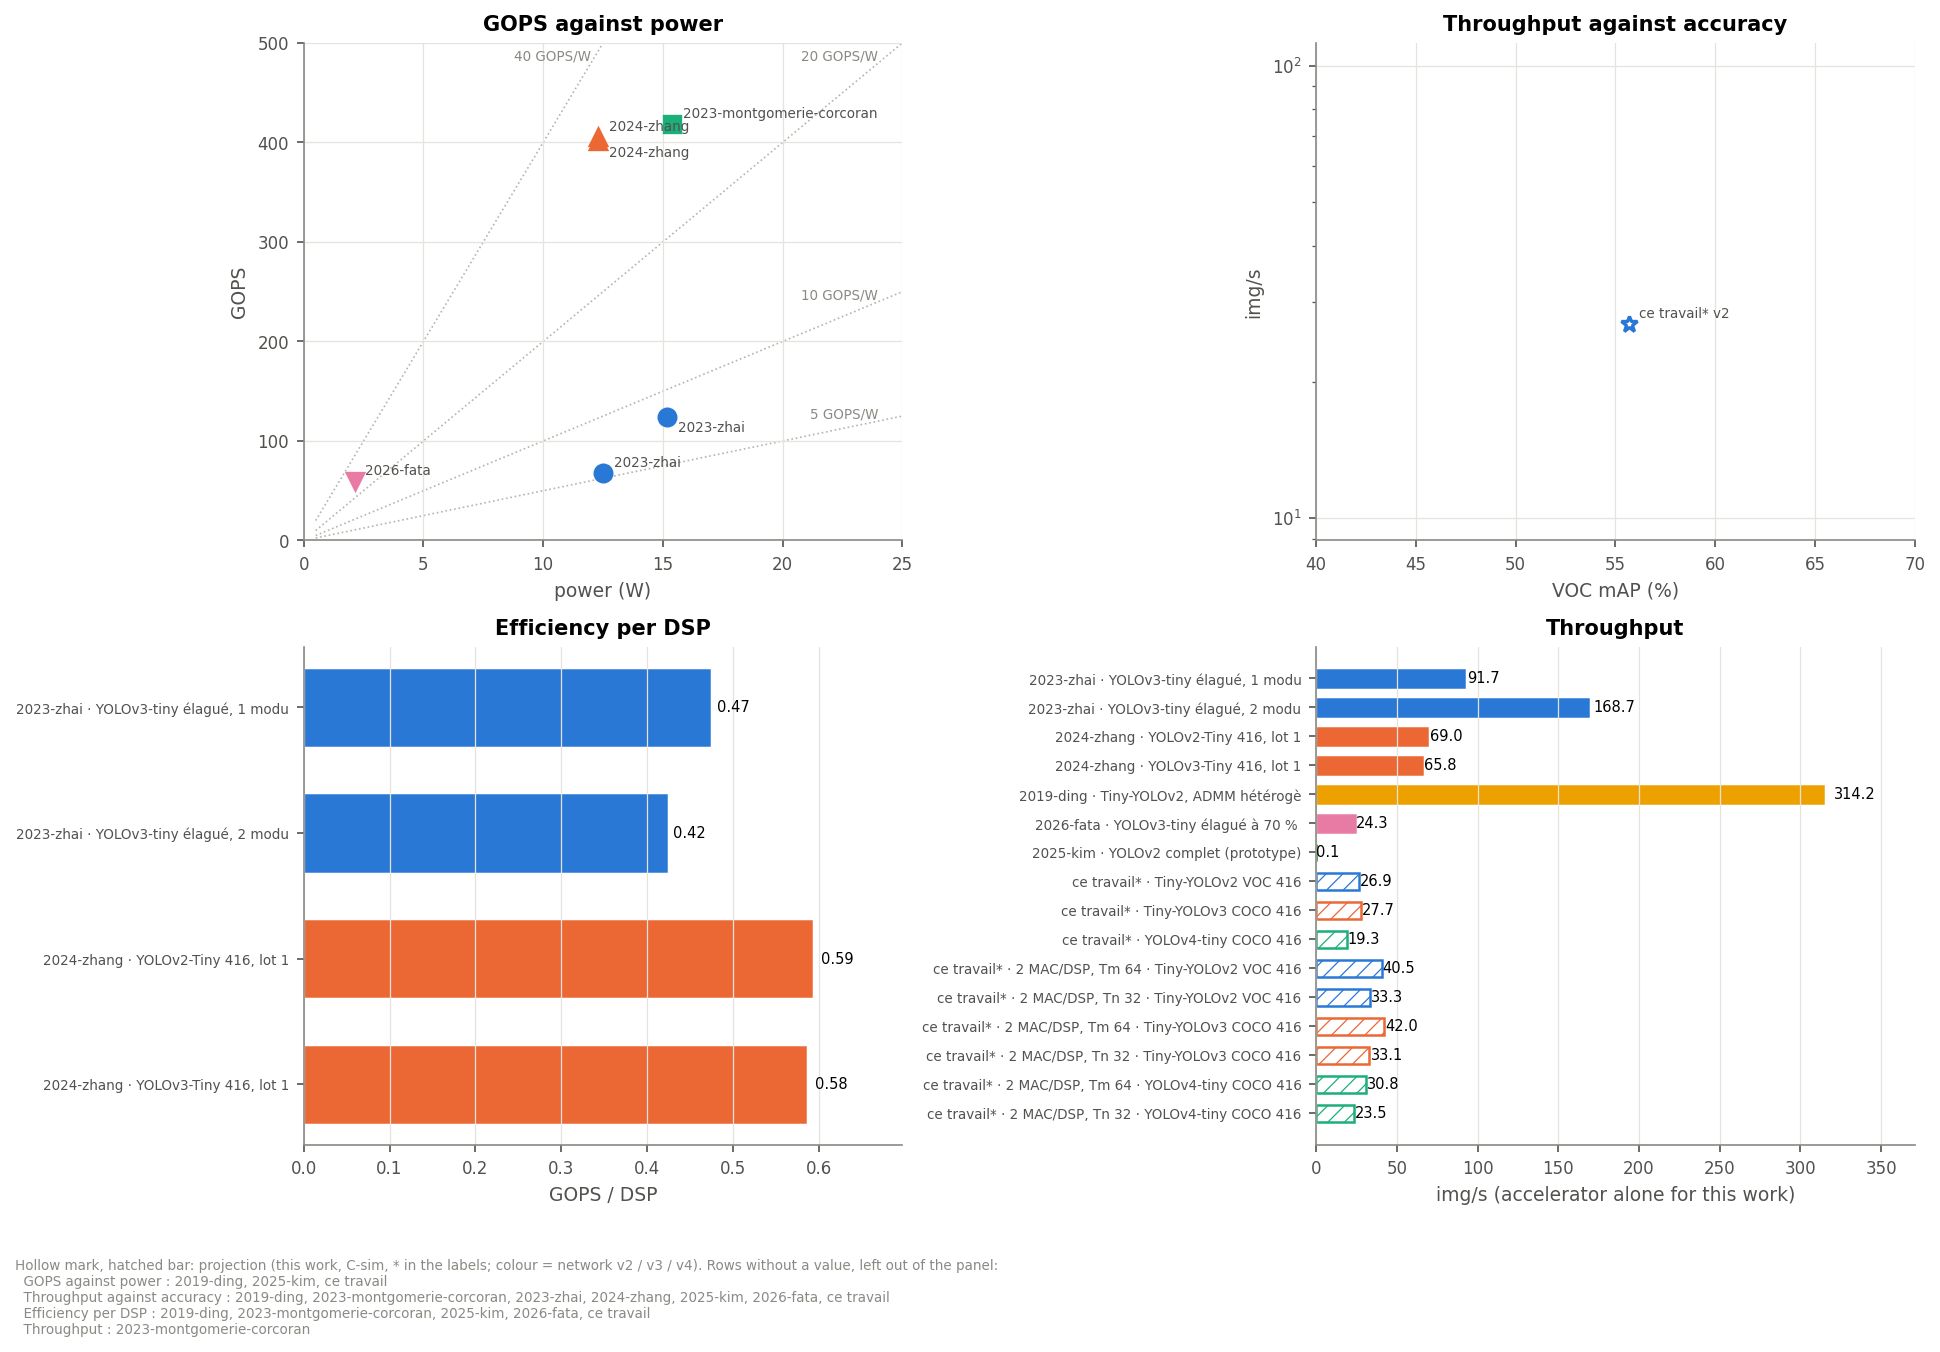
\includegraphics[width=\linewidth,height=0.42\textheight,keepaspectratio]{../../results/figures/resultats/etat_art.png}
\caption{Comparaison aux accélérateurs publiés : GOPS et puissance, débit et mAP, GOPS par DSP (marque creuse : projection de ce travail). (\texttt{etat\_art})}
\label{fig:etat_art}
% python -m tools.figures etat_art
\end{figure}}
\expandafter\def\csname artfig:graphe/graphe_tiny-yolov2-voc\endcsname{%
\begin{figure}[htbp]
\centering
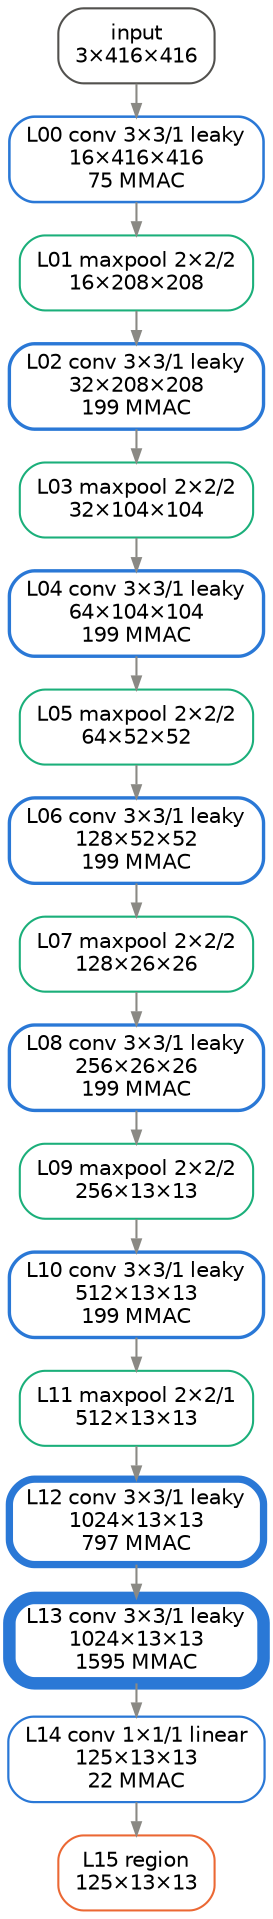
\includegraphics[width=\linewidth,height=0.42\textheight,keepaspectratio]{../../results/figures/modeles/graphe_tiny-yolov2-voc.png}
\caption{Graphe couche par couche (type, noyau et stride, forme de sortie C×H×W ; bord épais = beaucoup de MACs). (\texttt{graphe})}
\label{fig:graphe/graphe_tiny-yolov2-voc}
% python -m tools.figures graphe
\end{figure}}
\expandafter\def\csname artfig:fiche/fiche_tiny-yolov2-voc\endcsname{%
\begin{figure}[htbp]
\centering
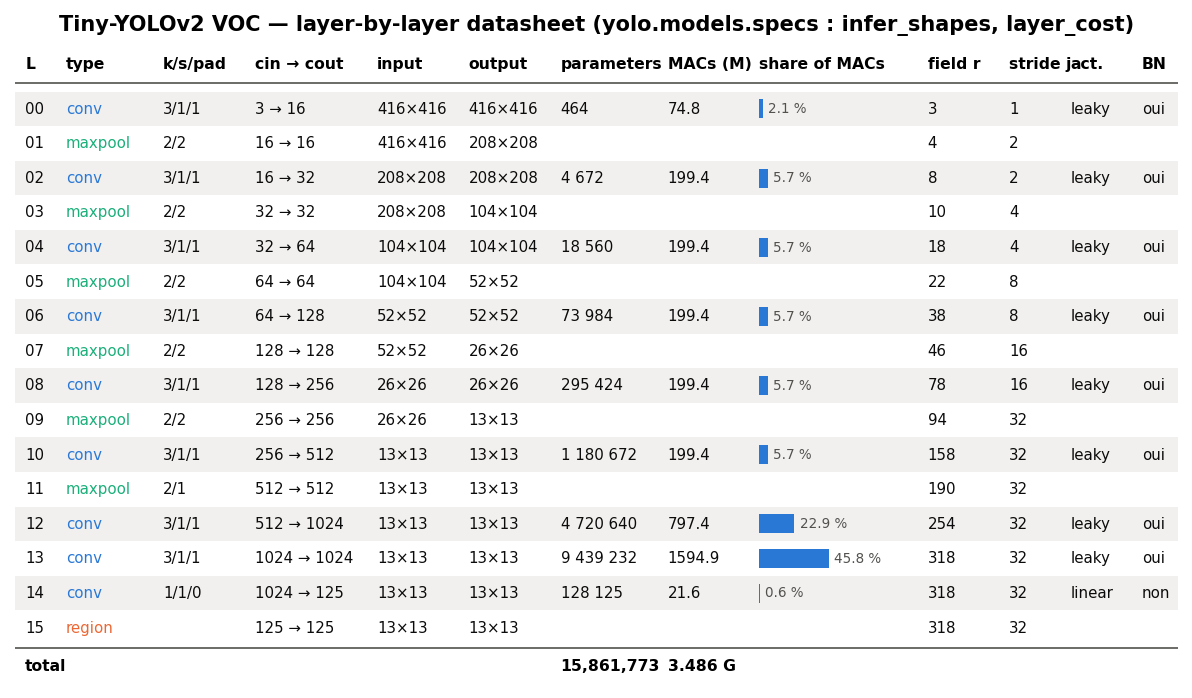
\includegraphics[width=\linewidth,height=0.42\textheight,keepaspectratio]{../../results/figures/reseaux/fiche_tiny-yolov2-voc.png}
\caption{Fiche couche par couche : type, noyau, formes, paramètres, MACs et leur part, champ réceptif et pas cumulé (CSV à côté de l'image). (\texttt{fiche})}
\label{fig:fiche/fiche_tiny-yolov2-voc}
% python -m tools.figures fiche
\end{figure}}
\expandafter\def\csname artfig:convolution\endcsname{%
\begin{figure}[htbp]
\centering
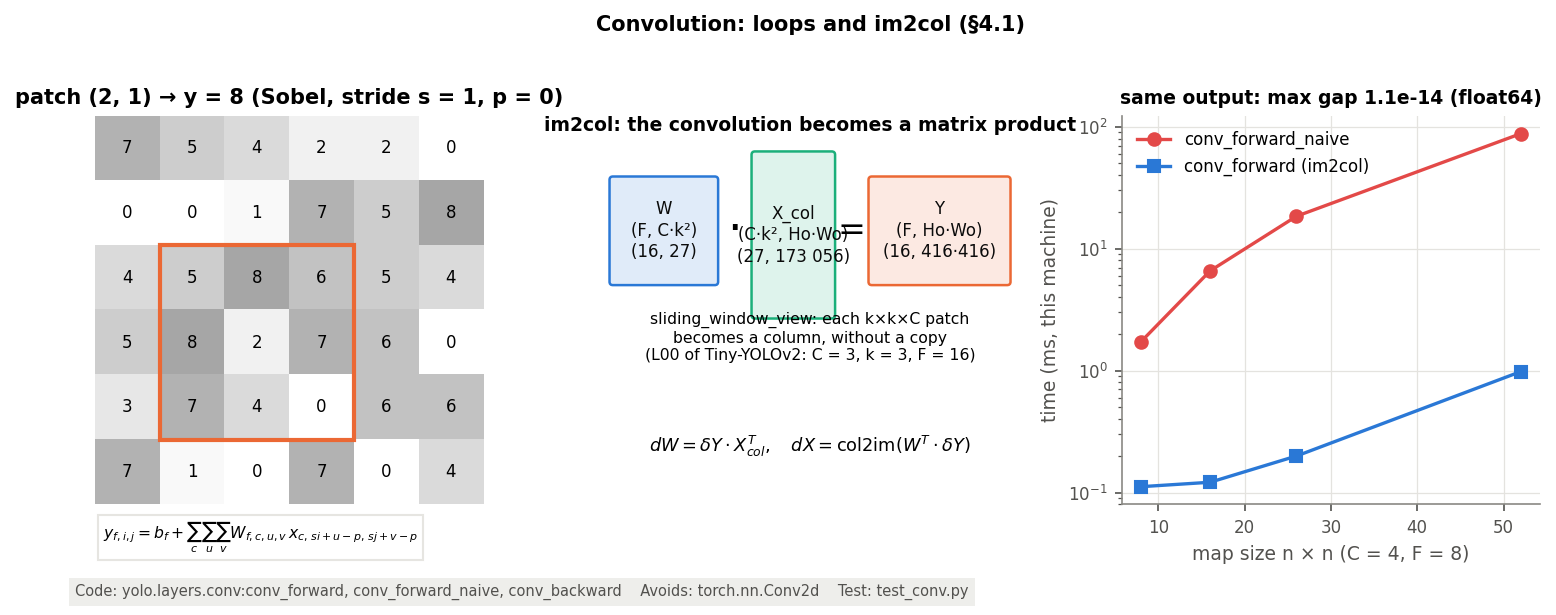
\includegraphics[width=\linewidth,height=0.42\textheight,keepaspectratio]{../../results/figures/maths/convolution.png}
\caption{Convolution : la formule sur un patch, le dépliage im2col en produit de matrices, et le temps des boucles face à im2col. (\texttt{convolution})}
\label{fig:convolution}
% python -m tools.figures convolution
\end{figure}}
\expandafter\def\csname artfig:retropropagation\endcsname{%
\begin{figure}[htbp]
\centering
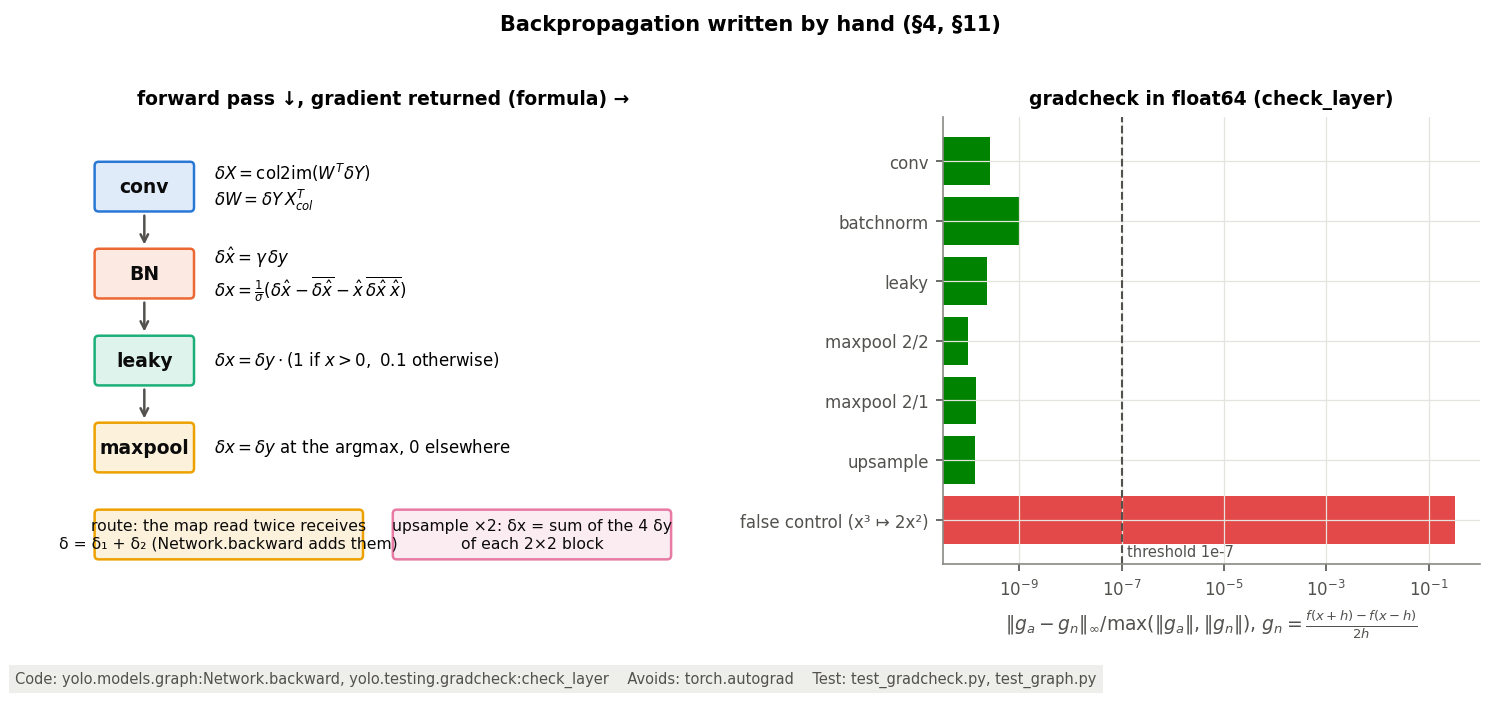
\includegraphics[width=\linewidth,height=0.42\textheight,keepaspectratio]{../../results/figures/maths/retropropagation.png}
\caption{Rétropropagation écrite à la main : formule du gradient renvoyé par chaque couche, puis l'erreur du gradcheck par couche face au seuil 1e-7. (\texttt{retropropagation})}
\label{fig:retropropagation}
% python -m tools.figures retropropagation
\end{figure}}
\expandafter\def\csname artfig:perte\endcsname{%
\begin{figure}[htbp]
\centering
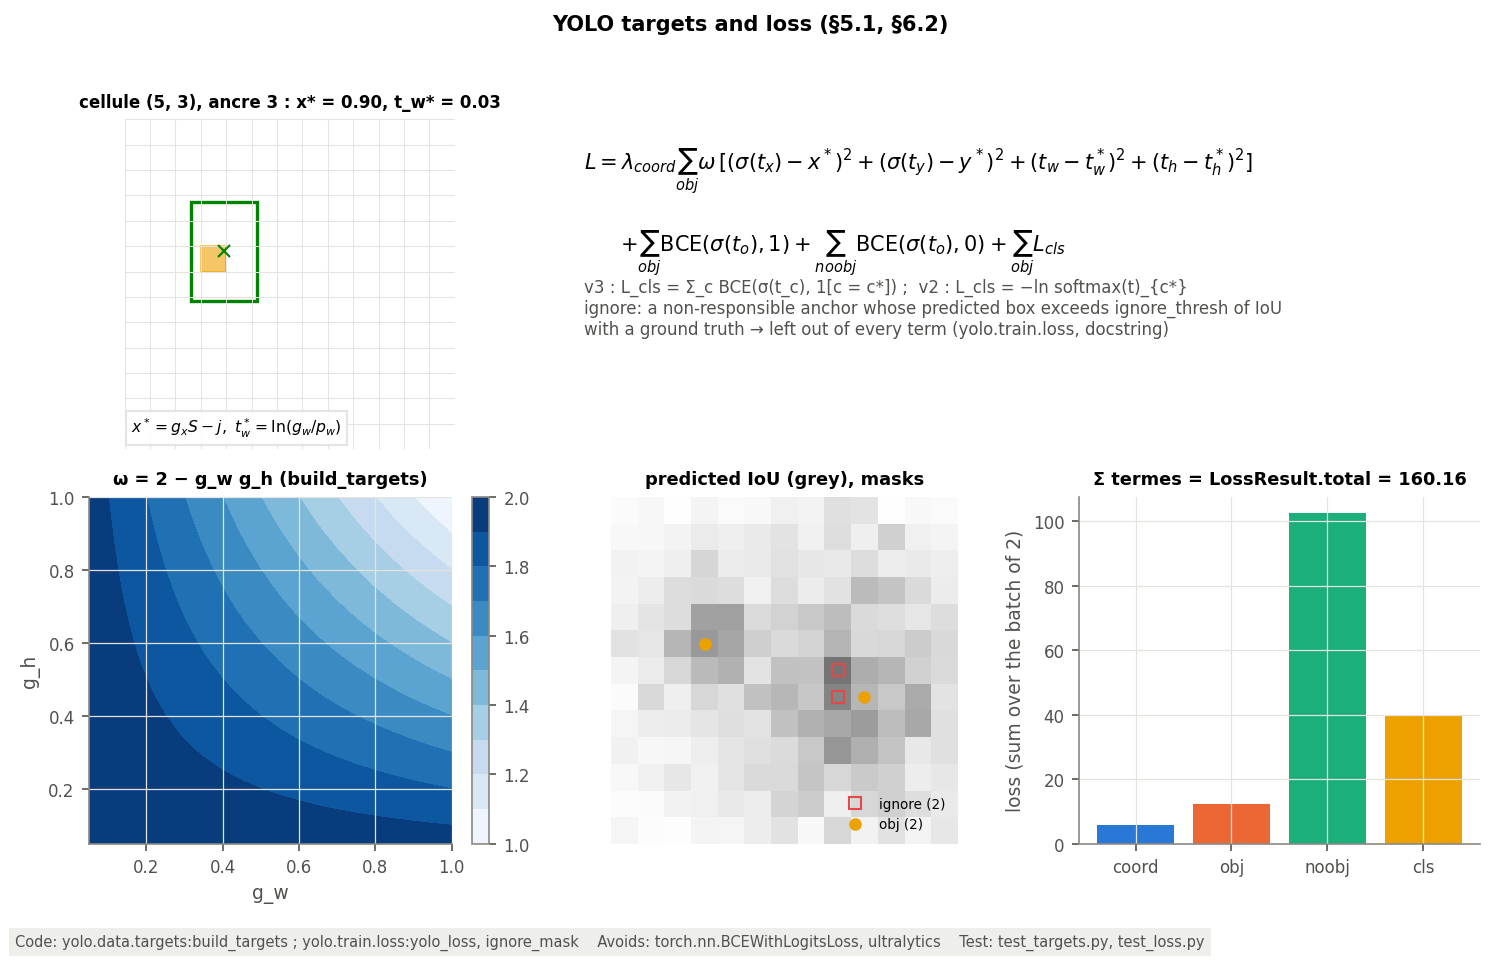
\includegraphics[width=\linewidth,height=0.42\textheight,keepaspectratio]{../../results/figures/maths/perte.png}
\caption{Cibles et perte YOLO : encodage d'une vérité, la perte terme par terme, le poids $\omega$ = 2 − g\_w g\_h, le masque ignore et la part de chaque terme sur un lot. (\texttt{perte})}
\label{fig:perte}
% python -m tools.figures perte
\end{figure}}
\expandafter\def\csname artfig:pr/pr_variantes\endcsname{%
\begin{figure}[htbp]
\centering
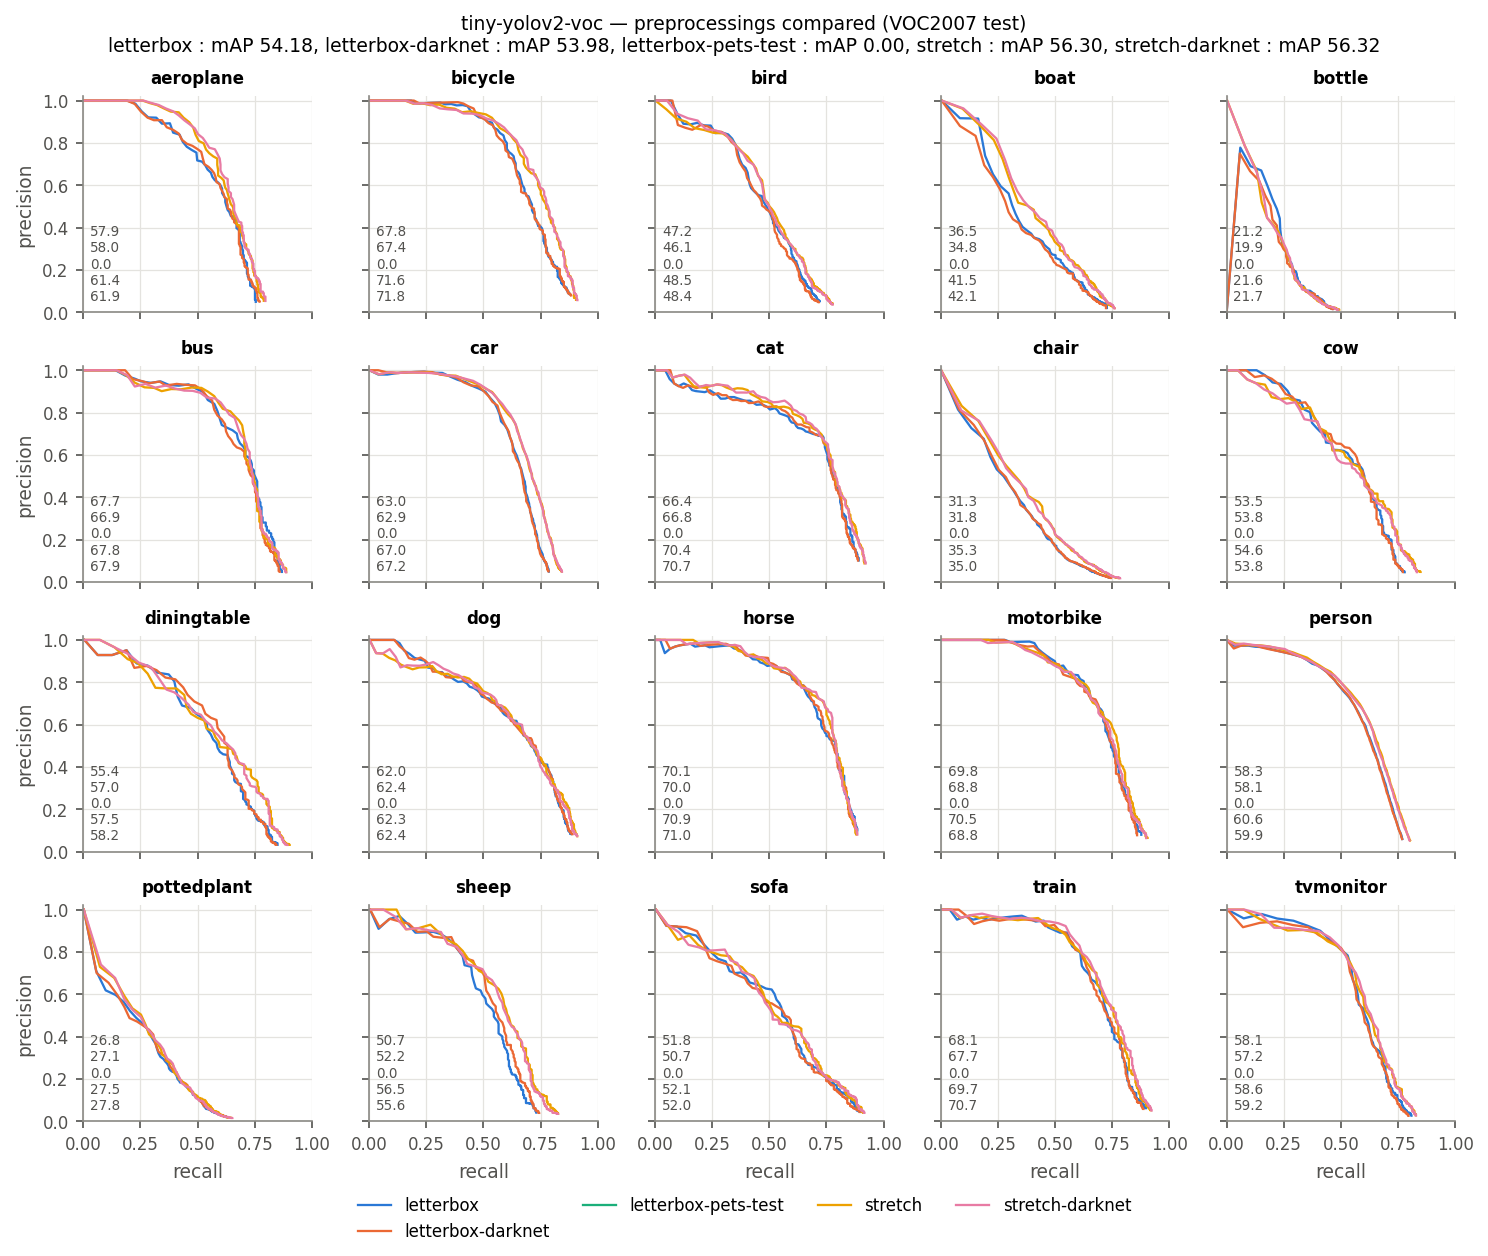
\includegraphics[width=\linewidth,height=0.42\textheight,keepaspectratio]{../../results/figures/resultats/pr_variantes.png}
\caption{Courbes précision-rappel par classe (11 points VOC07) pour chaque prétraitement évalué, puis les quatre superposées. (\texttt{pr})}
\label{fig:pr/pr_variantes}
% python -m tools.figures pr
\end{figure}}
\expandafter\def\csname artfig:nms_map\endcsname{%
\begin{figure}[htbp]
\centering
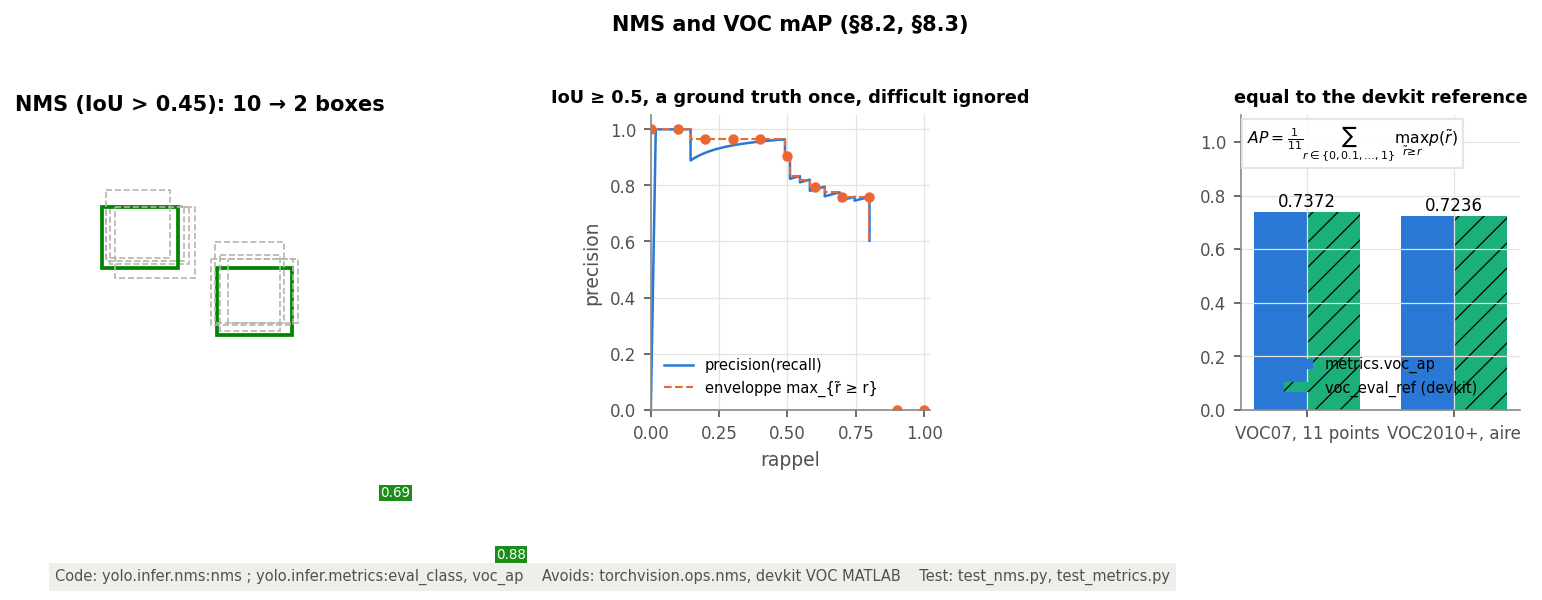
\includegraphics[width=\linewidth,height=0.42\textheight,keepaspectratio]{../../results/figures/maths/nms_map.png}
\caption{NMS pas à pas, appariement détections / vérités et courbe précision-rappel, AP VOC07 sur 11 points face à l'aire sous l'enveloppe, égale à la référence du devkit. (\texttt{nms\_map})}
\label{fig:nms_map}
% python -m tools.figures nms_map
\end{figure}}
\expandafter\def\csname artfig:quantification\endcsname{%
\begin{figure}[htbp]
\centering
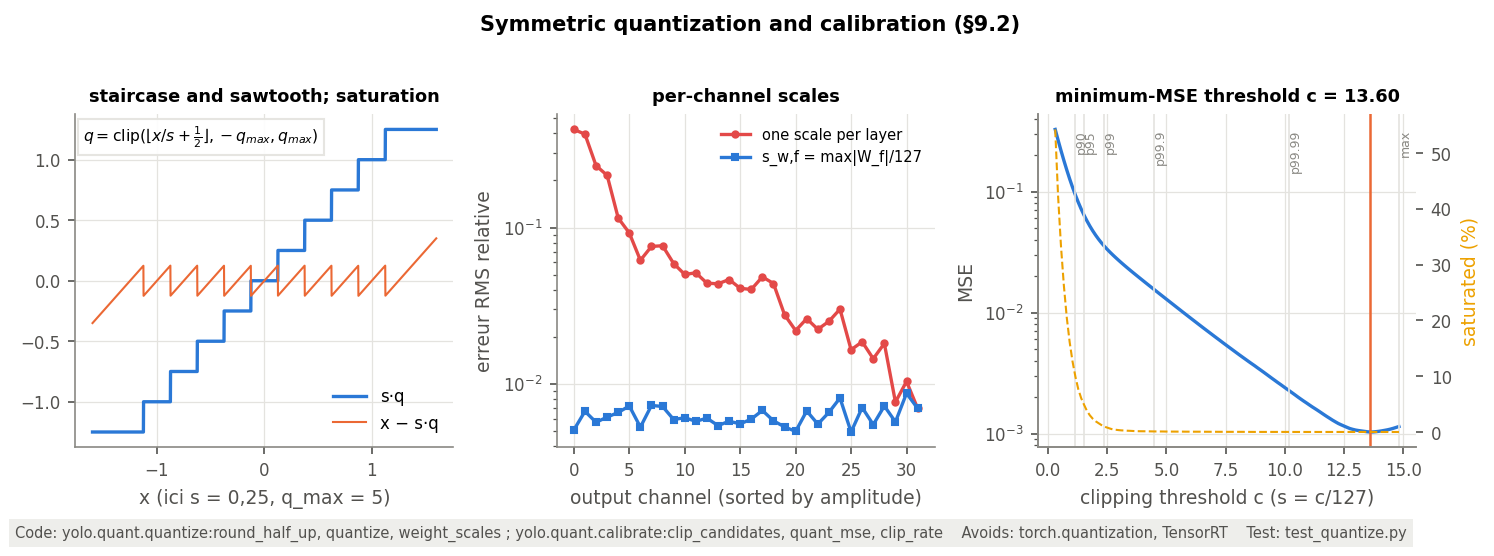
\includegraphics[width=\linewidth,height=0.42\textheight,keepaspectratio]{../../results/figures/maths/quantification.png}
\caption{Quantification symétrique : l'escalier et son erreur, échelles par canal face à une échelle par couche, choix du seuil d'écrêtage par la MSE. (\texttt{quantification})}
\label{fig:quantification}
% python -m tools.figures quantification
\end{figure}}
\expandafter\def\csname artfig:entier\endcsname{%
\begin{figure}[htbp]
\centering
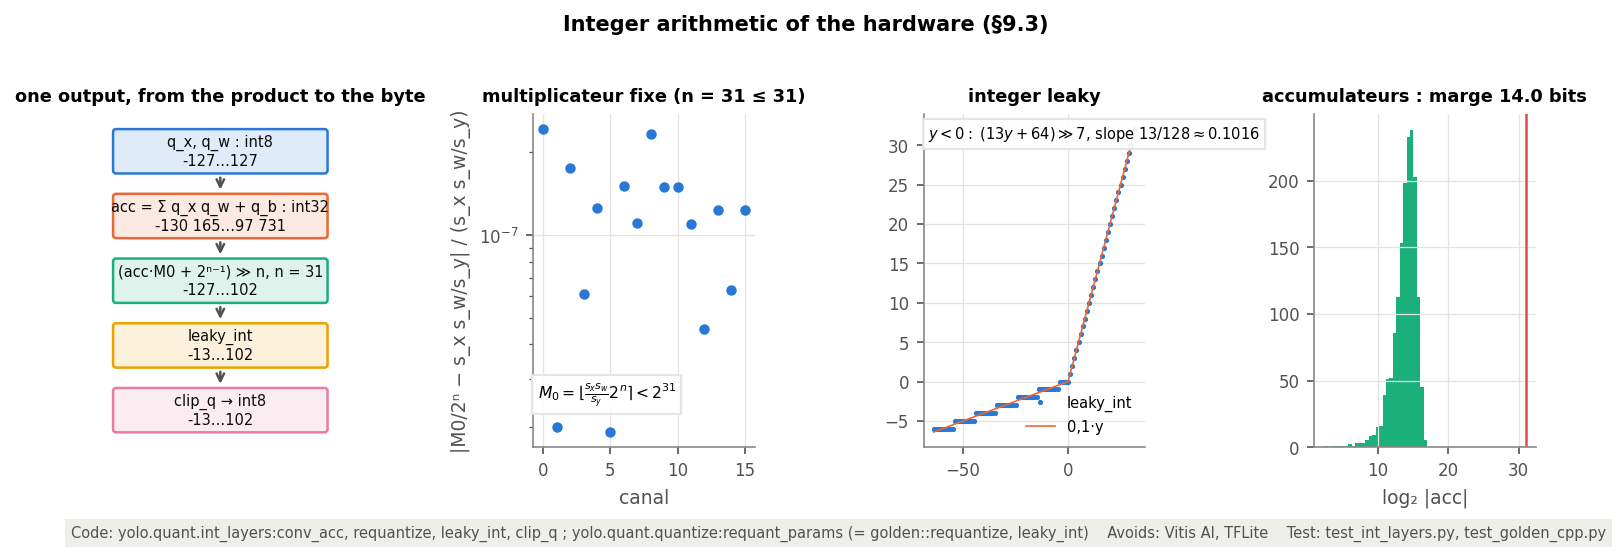
\includegraphics[width=\linewidth,height=0.42\textheight,keepaspectratio]{../../results/figures/maths/entier.png}
\caption{Arithmétique entière du matériel : chaîne d'une sortie, multiplicateur fixe M0/2$^n$, leaky entière 13/128 et marge des accumulateurs int32. (\texttt{entier})}
\label{fig:entier}
% python -m tools.figures entier
\end{figure}}
\expandafter\def\csname artfig:calibration/calibration_tiny-yolov2-voc\endcsname{%
\begin{figure}[htbp]
\centering
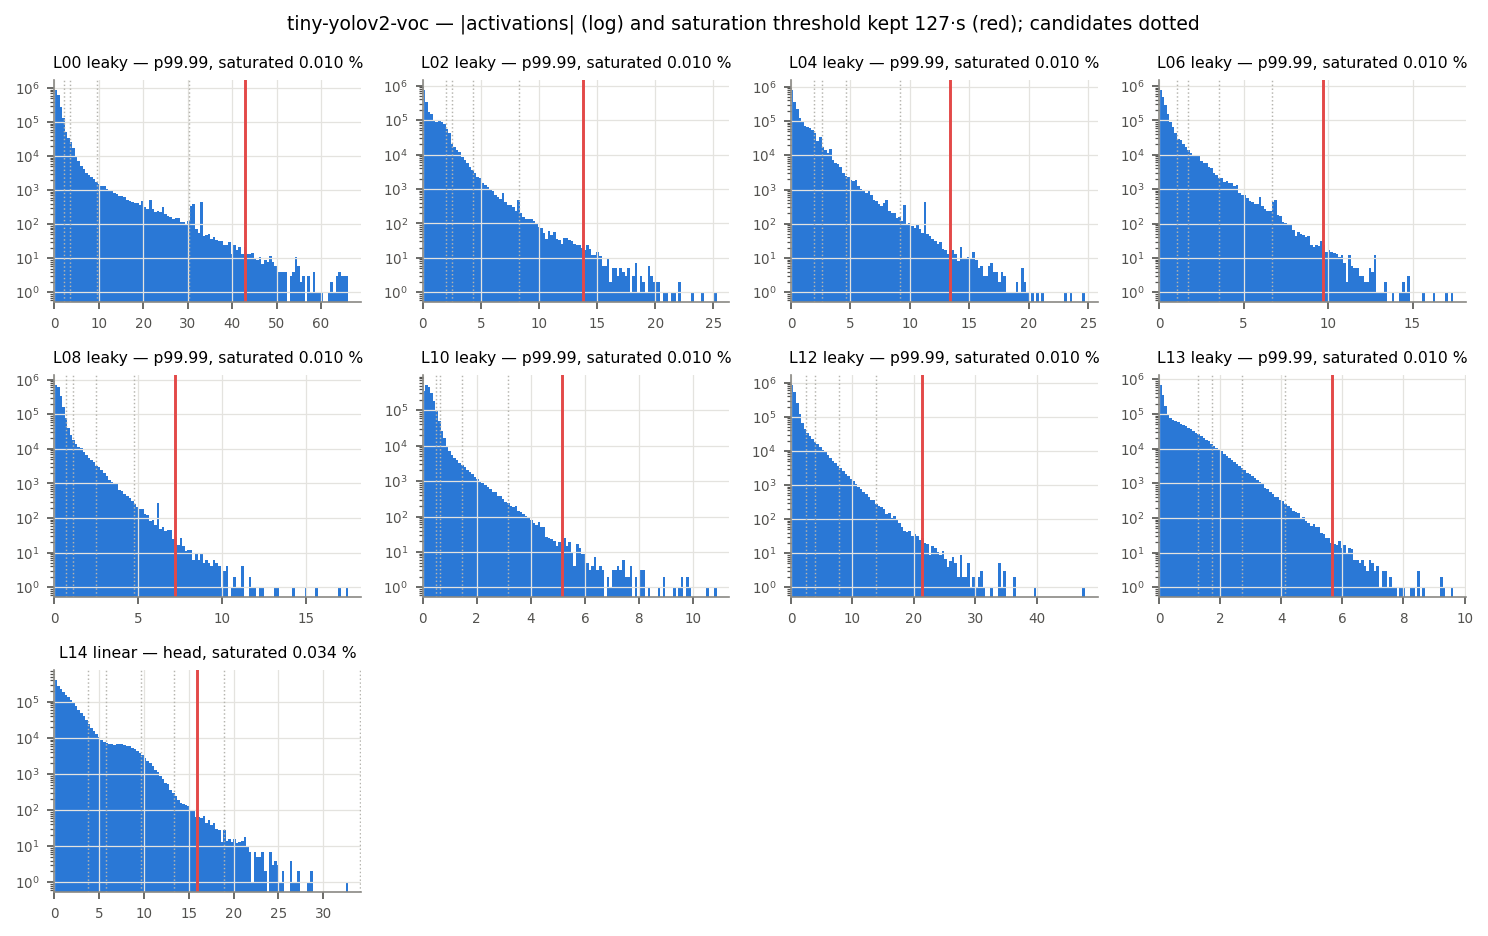
\includegraphics[width=\linewidth,height=0.42\textheight,keepaspectratio]{../../results/figures/resultats/calibration_tiny-yolov2-voc.png}
\caption{Distribution des activations par couche et seuil de saturation retenu par la calibration ; échelles des poids par canal. (\texttt{calibration})}
\label{fig:calibration/calibration_tiny-yolov2-voc}
% python -m tools.figures calibration
\end{figure}}
\expandafter\def\csname artfig:erreur_couches/erreur_couches_tiny-yolov2-voc\endcsname{%
\begin{figure}[htbp]
\centering
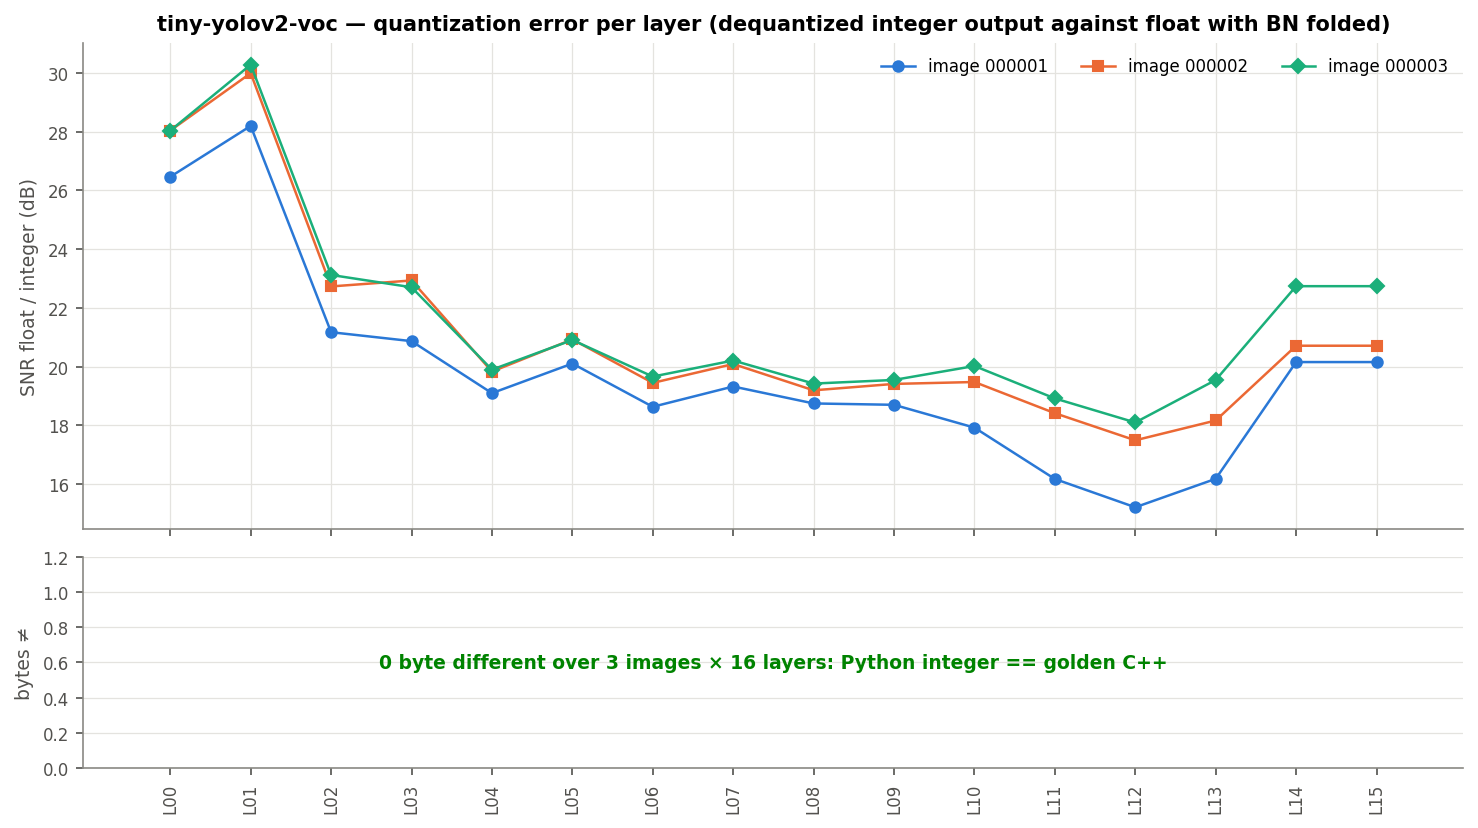
\includegraphics[width=\linewidth,height=0.42\textheight,keepaspectratio]{../../results/figures/resultats/erreur_couches_tiny-yolov2-voc.png}
\caption{SNR par couche entre le flottant et l'entier déquantifié, et écart entier Python $\leftrightarrow$ golden C++ (0 partout : bit-exact). (\texttt{erreur\_couches})}
\label{fig:erreur_couches/erreur_couches_tiny-yolov2-voc}
% python -m tools.figures erreur_couches
\end{figure}}
\expandafter\def\csname artfig:chaine_verif\endcsname{%
\begin{figure}[htbp]
\centering
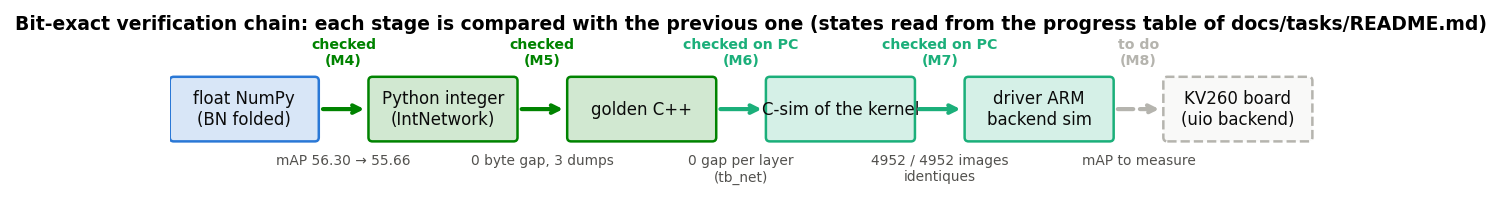
\includegraphics[width=\linewidth,height=0.42\textheight,keepaspectratio]{../../results/figures/materiel/chaine_verif.png}
\caption{Chaîne de vérification bit-exact, du flottant NumPy à la carte : critère et état de chaque passage. (\texttt{chaine\_verif})}
\label{fig:chaine_verif}
% python -m tools.figures chaine_verif
\end{figure}}
\expandafter\def\csname artfig:moteur\endcsname{%
\begin{figure}[htbp]
\centering
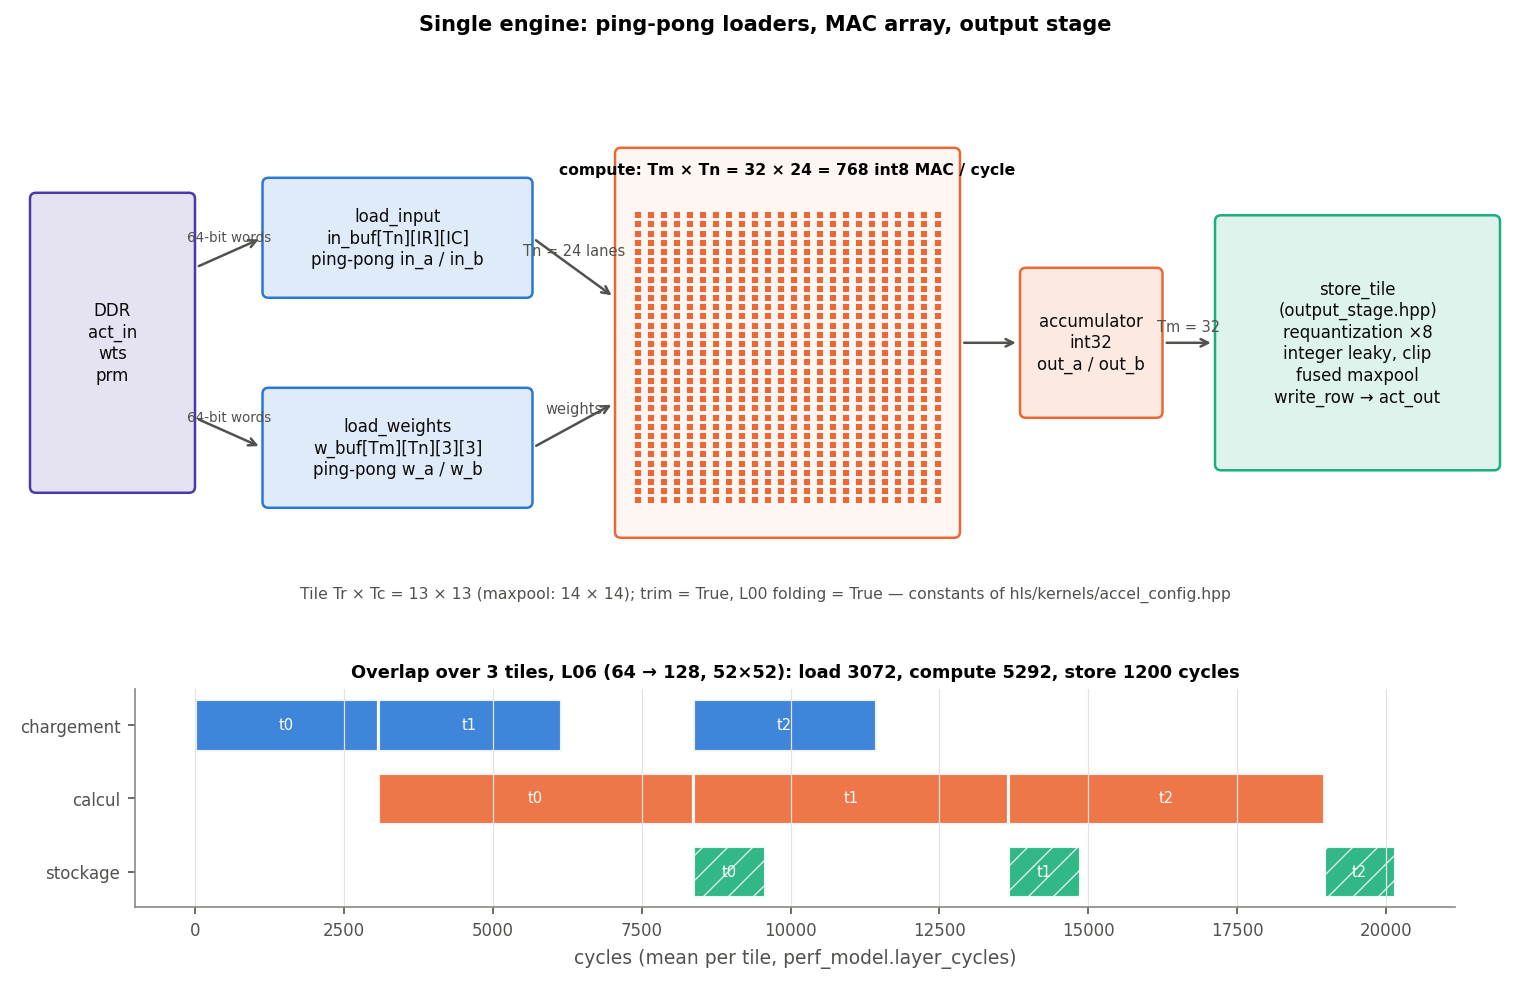
\includegraphics[width=\linewidth,height=0.42\textheight,keepaspectratio]{../../results/figures/materiel/moteur.png}
\caption{Moteur unique : chargeurs ping-pong, réseau Tm × Tn de MACs, accumulateur, étage de sortie, et chronogramme du recouvrement sur 3 tuiles. (\texttt{moteur})}
\label{fig:moteur}
% python -m tools.figures moteur
\end{figure}}
\expandafter\def\csname artfig:tuilage\endcsname{%
\begin{figure}[htbp]
\centering
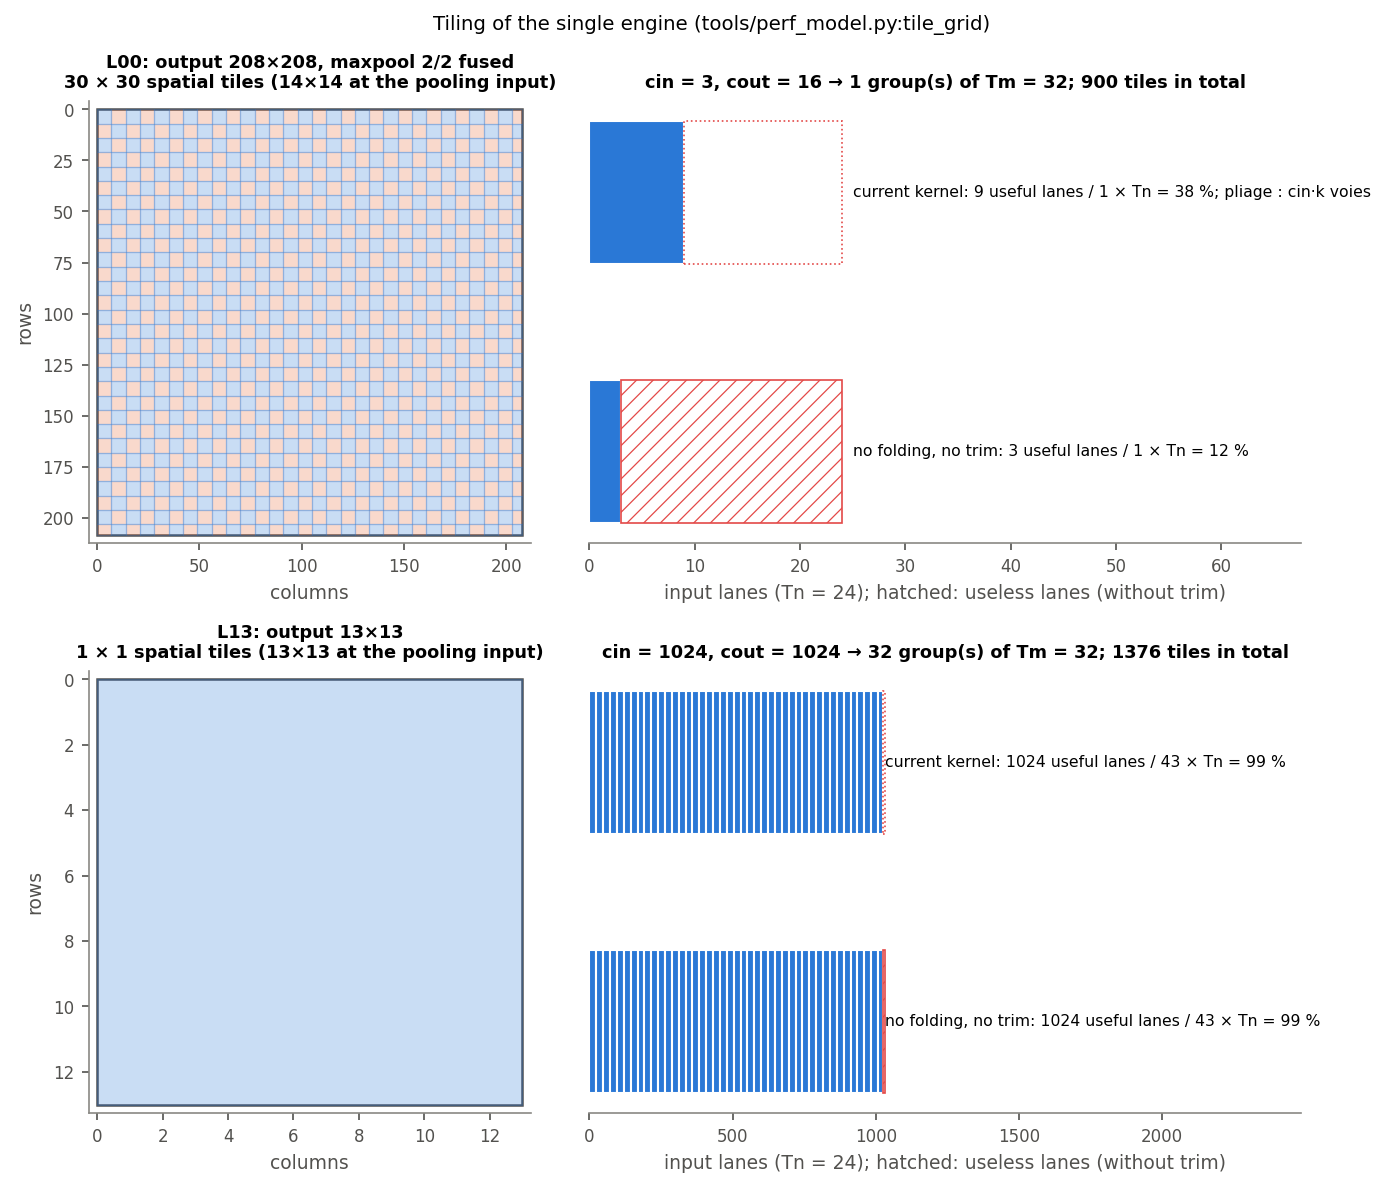
\includegraphics[width=\linewidth,height=0.42\textheight,keepaspectratio]{../../results/figures/materiel/tuilage.png}
\caption{Tuilage de deux couches : tuiles spatiales et voies d'entrée, avec le pliage de L00 (cin = 3) et la couche 13×13 couverte par une seule tuile. (\texttt{tuilage})}
\label{fig:tuilage}
% python -m tools.figures tuilage
\end{figure}}
\expandafter\def\csname artfig:soc\endcsname{%
\begin{figure}[htbp]
\centering
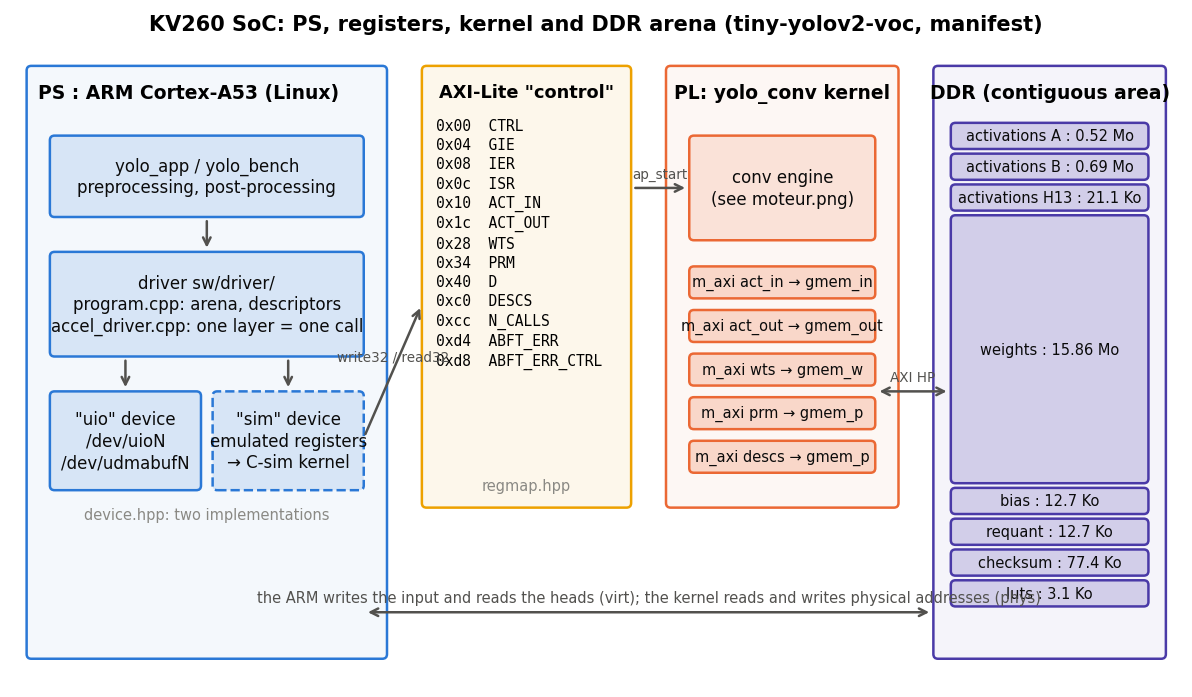
\includegraphics[width=\linewidth,height=0.42\textheight,keepaspectratio]{../../results/figures/materiel/soc.png}
\caption{Schéma du SoC : application et driver sur l'ARM, registres AXI-Lite, ports m\_axi du noyau et découpage de l'arène DDR. (\texttt{soc})}
\label{fig:soc}
% python -m tools.figures soc
\end{figure}}
\expandafter\def\csname artfig:cascade_m10\endcsname{%
\begin{figure}[htbp]
\centering
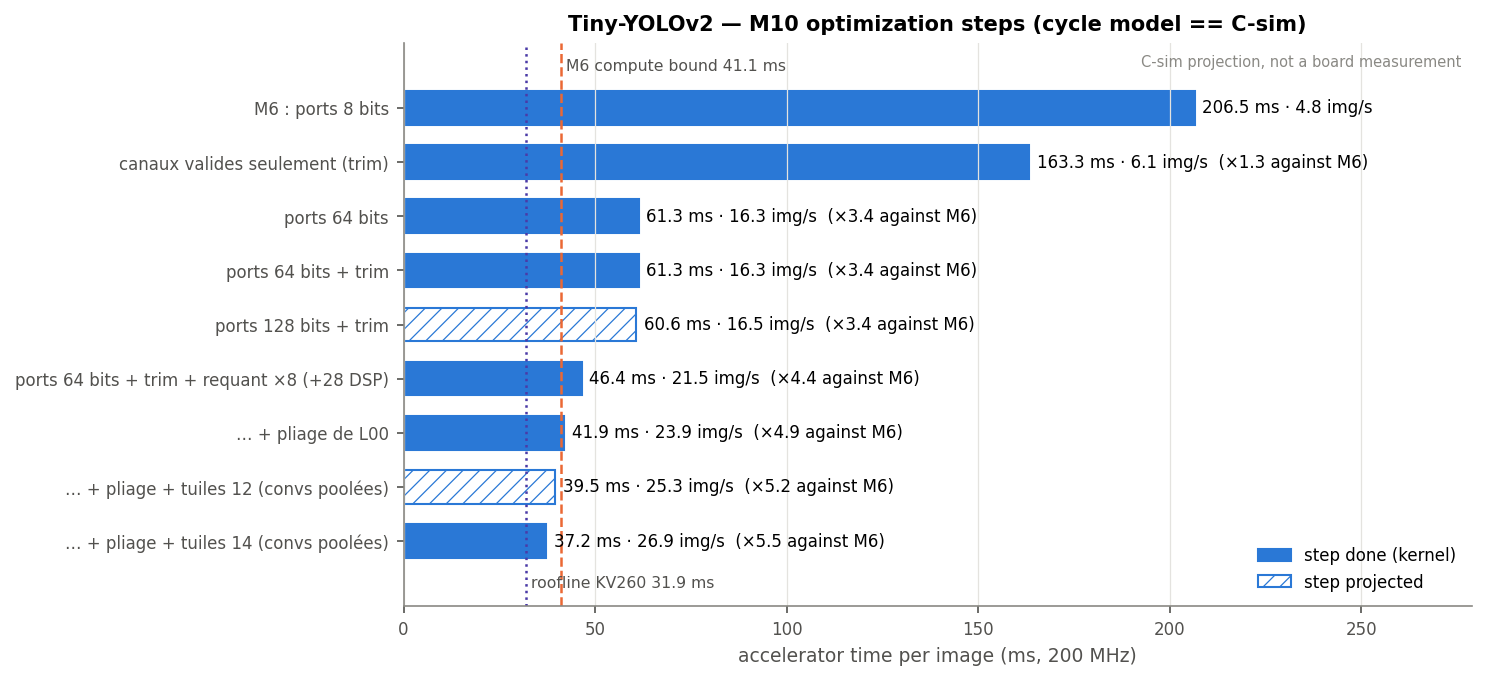
\includegraphics[width=\linewidth,height=0.42\textheight,keepaspectratio]{../../results/figures/resultats/cascade_m10.png}
\caption{Temps par image de Tiny-YOLOv2 à chaque piste d'optimisation M10, face à la borne de calcul et au roofline KV260. (\texttt{cascade\_m10})}
\label{fig:cascade_m10}
% python -m tools.figures cascade_m10
\end{figure}}
\expandafter\def\csname artfig:roofline_couches/roofline_couches_kv260\endcsname{%
\begin{figure}[htbp]
\centering
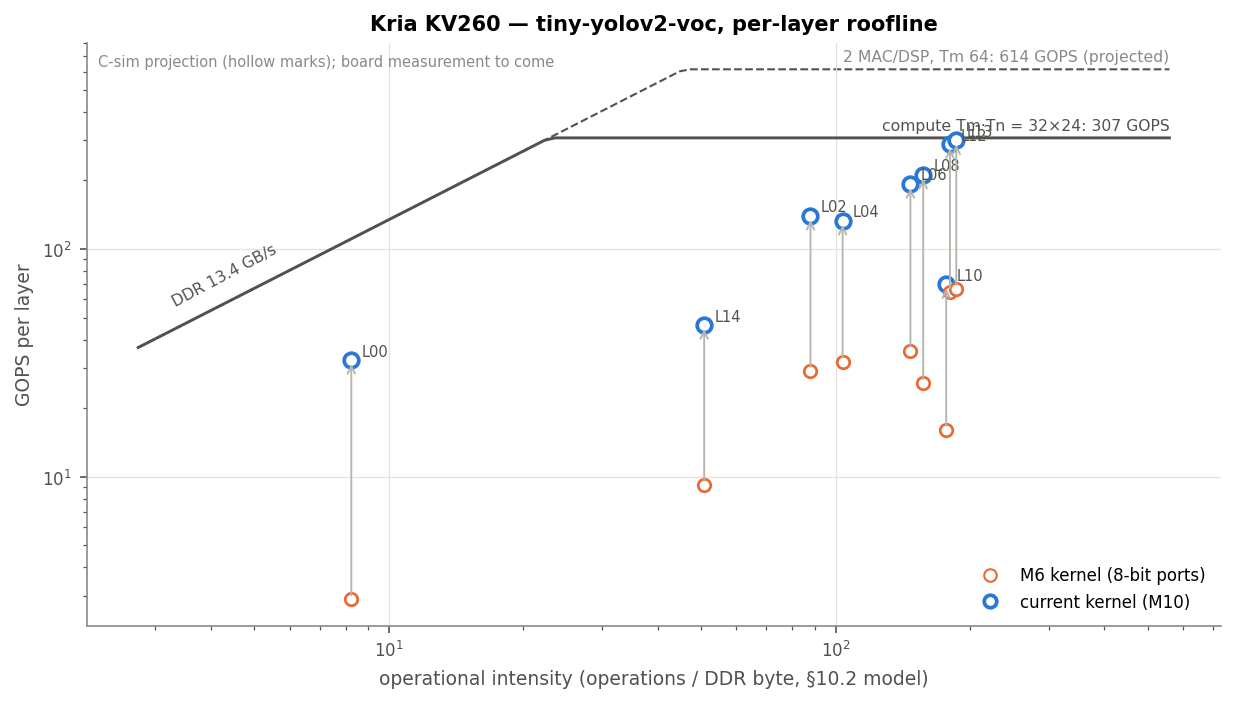
\includegraphics[width=\linewidth,height=0.42\textheight,keepaspectratio]{../../results/figures/resultats/roofline_couches_kv260.png}
\caption{Roofline KV260 avec un point par couche de Tiny-YOLOv2, avant et après les optimisations M10. (\texttt{roofline\_couches})}
\label{fig:roofline_couches/roofline_couches_kv260}
% python -m tools.figures roofline_couches
\end{figure}}
\expandafter\def\csname artfig:cycles_couches\endcsname{%
\begin{figure}[htbp]
\centering
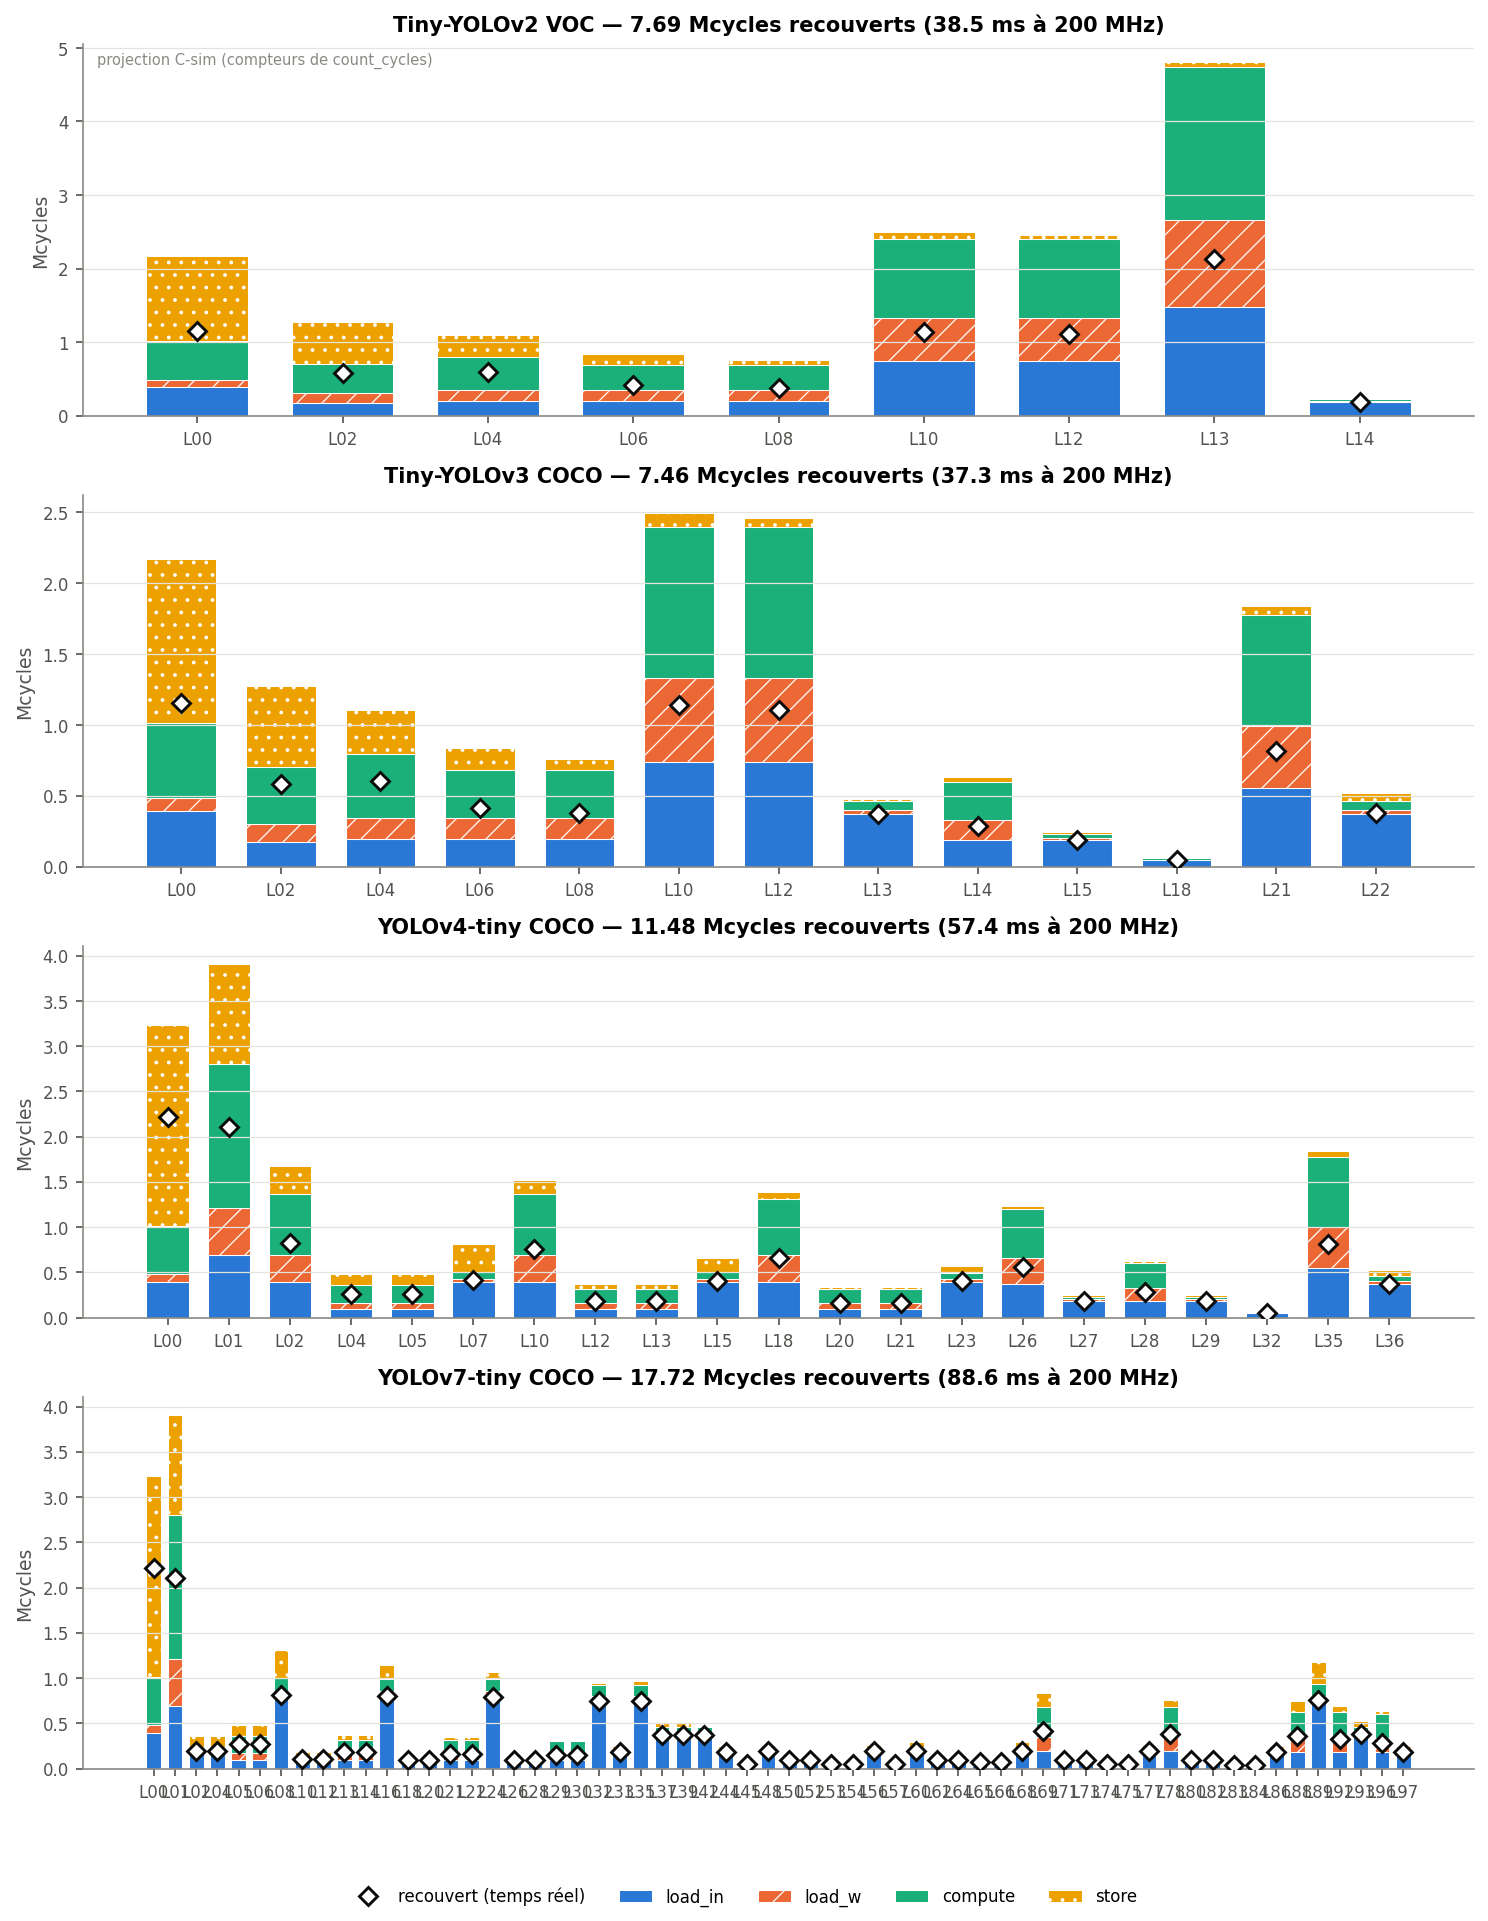
\includegraphics[width=\linewidth,height=0.42\textheight,keepaspectratio]{../../results/figures/resultats/cycles_couches.png}
\caption{Cycles par couche du noyau actuel, décomposés en chargements, calcul et stockage ; le losange donne le temps réel avec recouvrement. (\texttt{cycles\_couches})}
\label{fig:cycles_couches}
% python -m tools.figures cycles_couches
\end{figure}}
\expandafter\def\csname artfig:map_stades\endcsname{%
\begin{figure}[htbp]
\centering
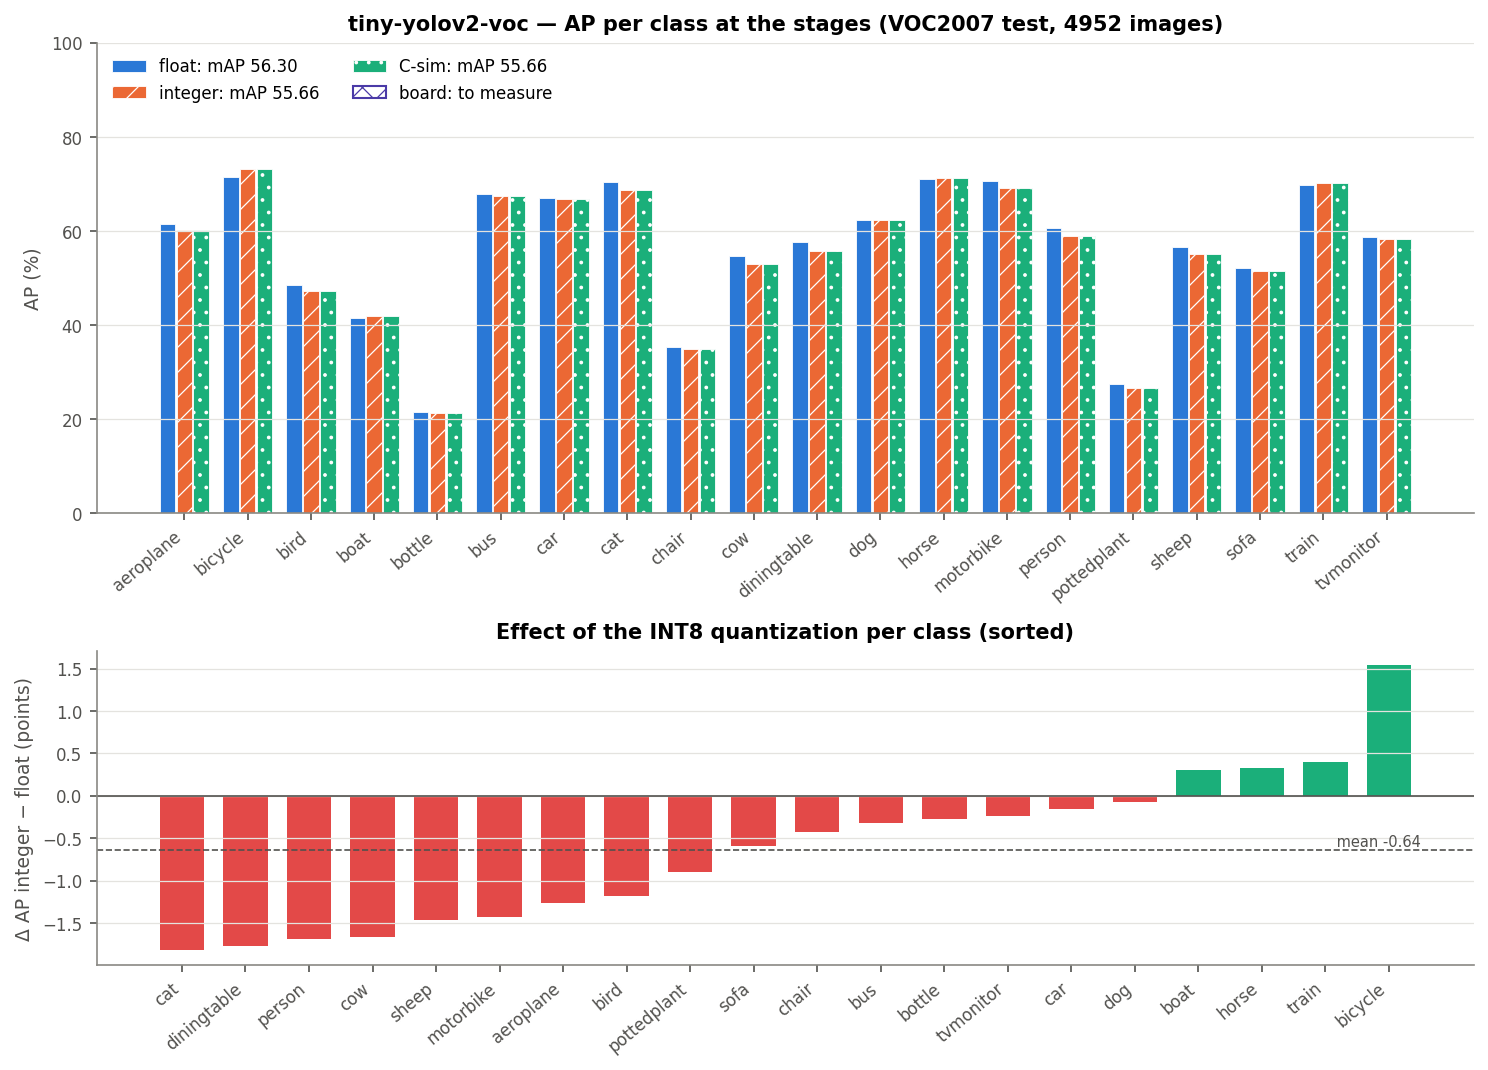
\includegraphics[width=\linewidth,height=0.42\textheight,keepaspectratio]{../../results/figures/resultats/map_stades.png}
\caption{AP par classe aux stades flottant, entier et C-sim (la carte quand elle sera mesurée), et écart entier − flottant trié. (\texttt{map\_stades})}
\label{fig:map_stades}
% python -m tools.figures map_stades
\end{figure}}
\expandafter\def\csname artfig:ressources\endcsname{%
\begin{figure}[htbp]
\centering
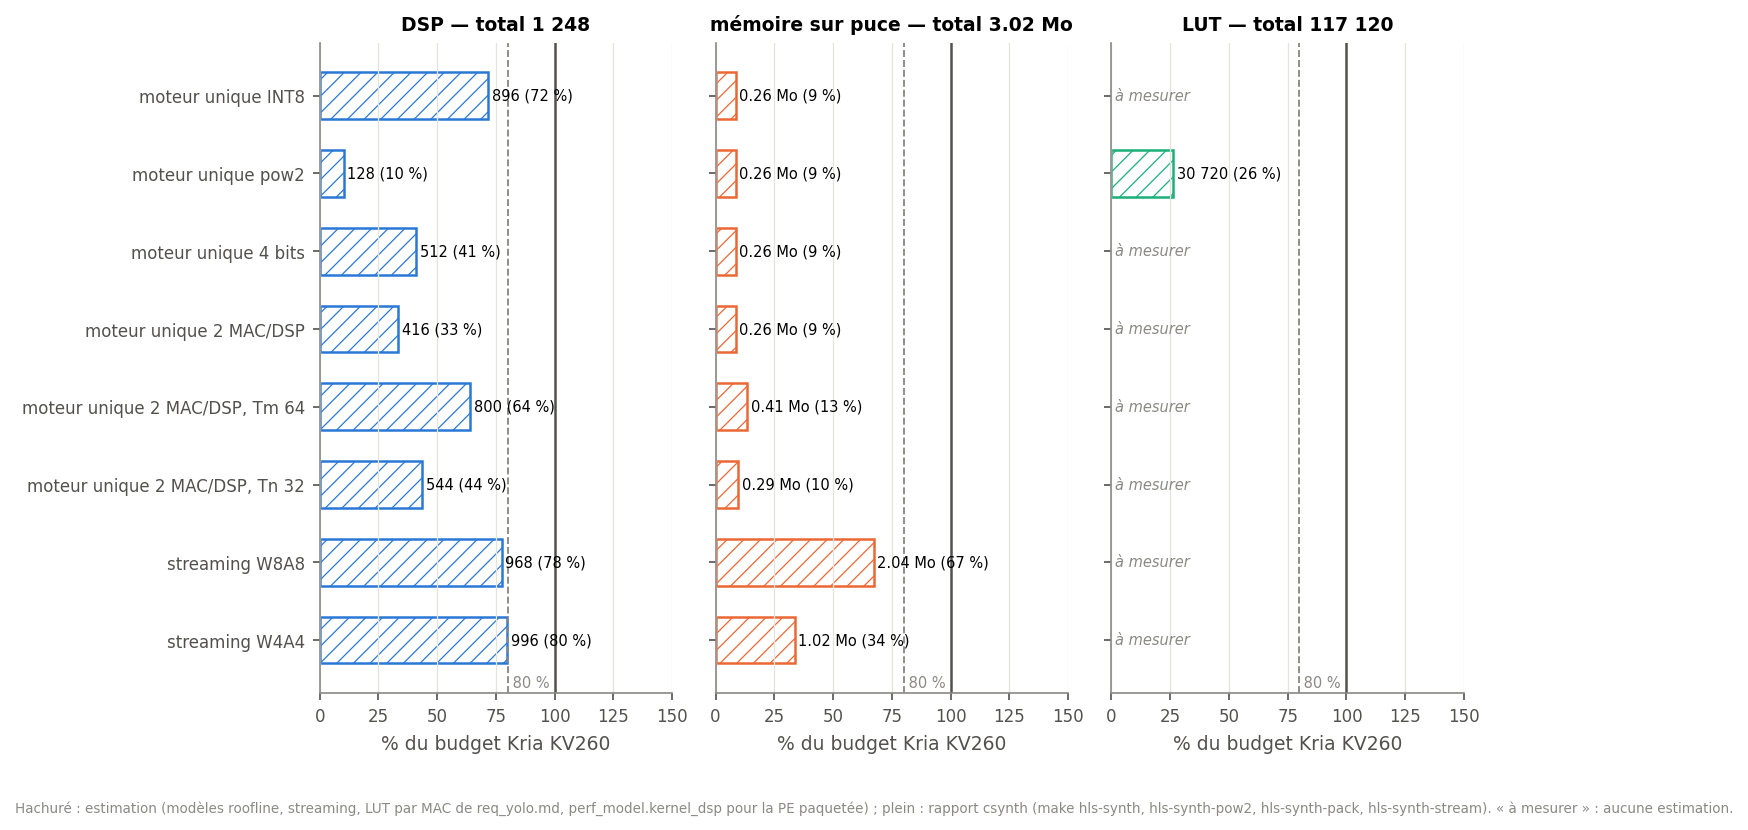
\includegraphics[width=\linewidth,height=0.42\textheight,keepaspectratio]{../../results/figures/resultats/ressources.png}
\caption{DSP, mémoire sur puce et LUT des architectures (moteur unique INT8, pow2 et 4 bits, streaming) face au budget de la KV260 ; hachuré : estimation, plein : synthèse. (\texttt{ressources})}
\label{fig:ressources}
% python -m tools.figures ressources
\end{figure}}
\expandafter\def\csname artfig:hw_postproc\endcsname{%
\begin{figure}[htbp]
\centering
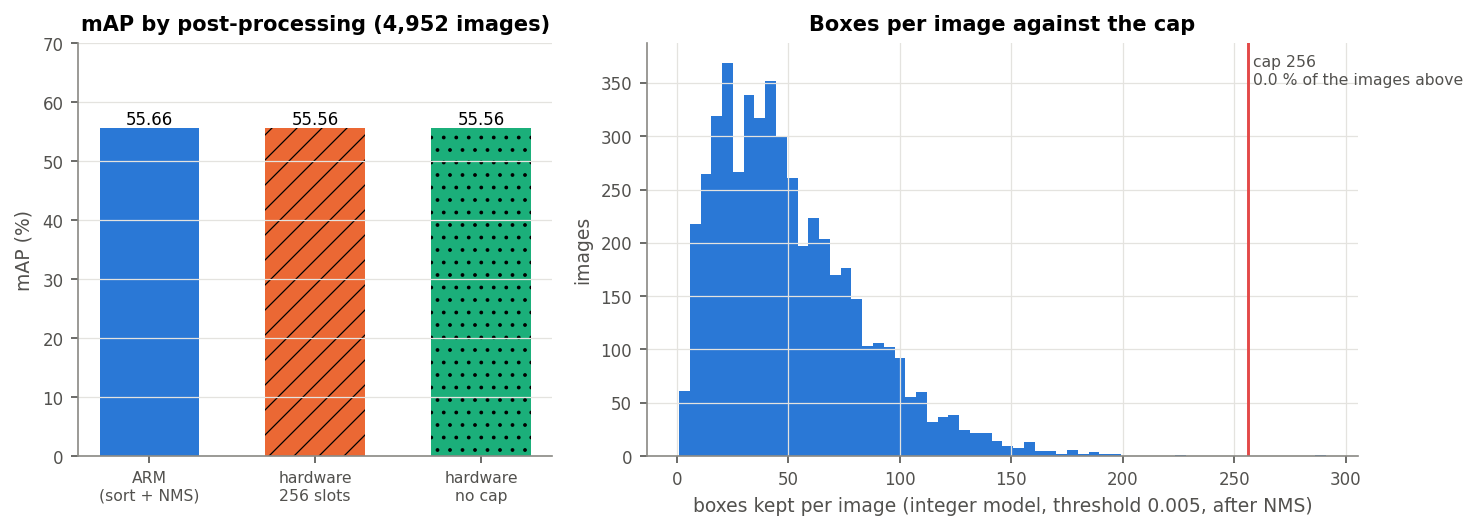
\includegraphics[width=\linewidth,height=0.42\textheight,keepaspectratio]{../../results/figures/resultats/hw_postproc.png}
\caption{mAP avec le post-traitement matériel, avec et sans plafond de boîtes, et nombre de boîtes par image face au plafond. (\texttt{hw\_postproc})}
\label{fig:hw_postproc}
% python -m tools.figures hw_postproc
\end{figure}}
\expandafter\def\csname artfig:map_formats\endcsname{%
\begin{figure}[htbp]
\centering
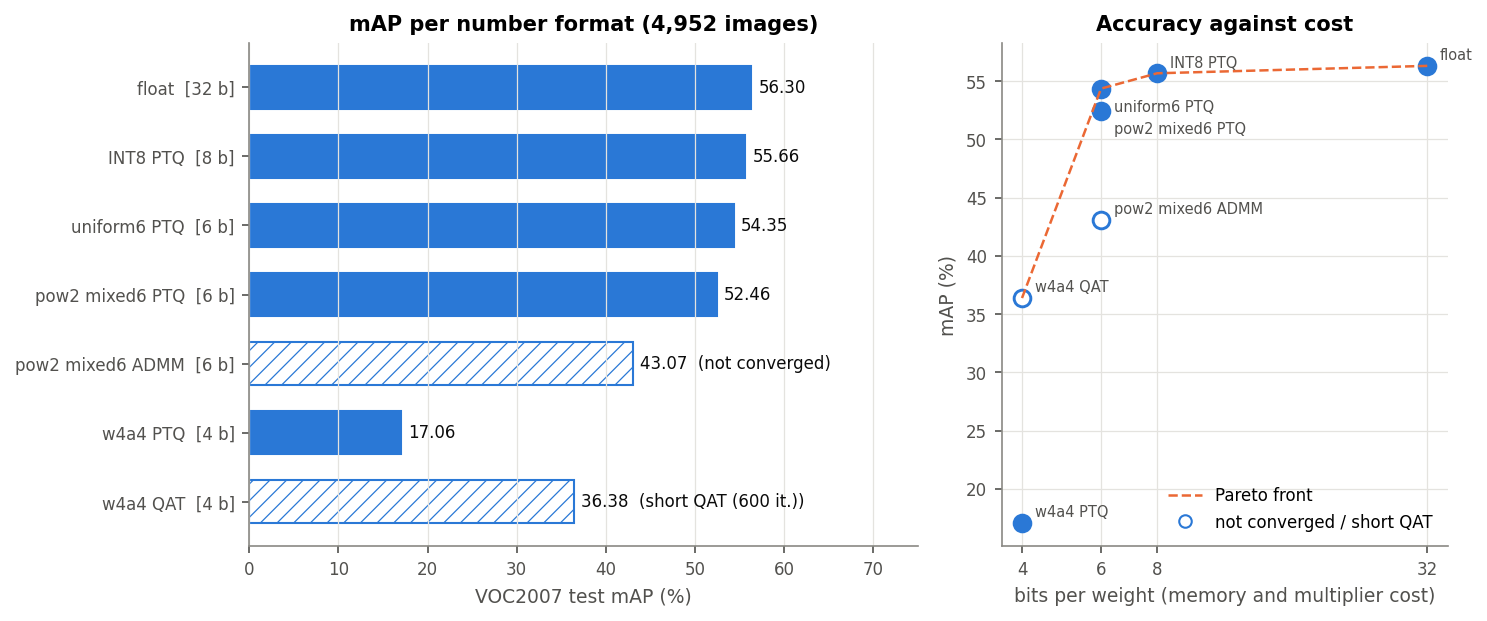
\includegraphics[width=\linewidth,height=0.42\textheight,keepaspectratio]{../../results/figures/resultats/map_formats.png}
\caption{mAP de Tiny-YOLOv2 selon le format des poids (flottant, INT8, puissances de 2, 4 bits), et frontière précision / bits. (\texttt{map\_formats})}
\label{fig:map_formats}
% python -m tools.figures map_formats
\end{figure}}
\expandafter\def\csname artfig:streaming\endcsname{%
\begin{figure}[htbp]
\centering
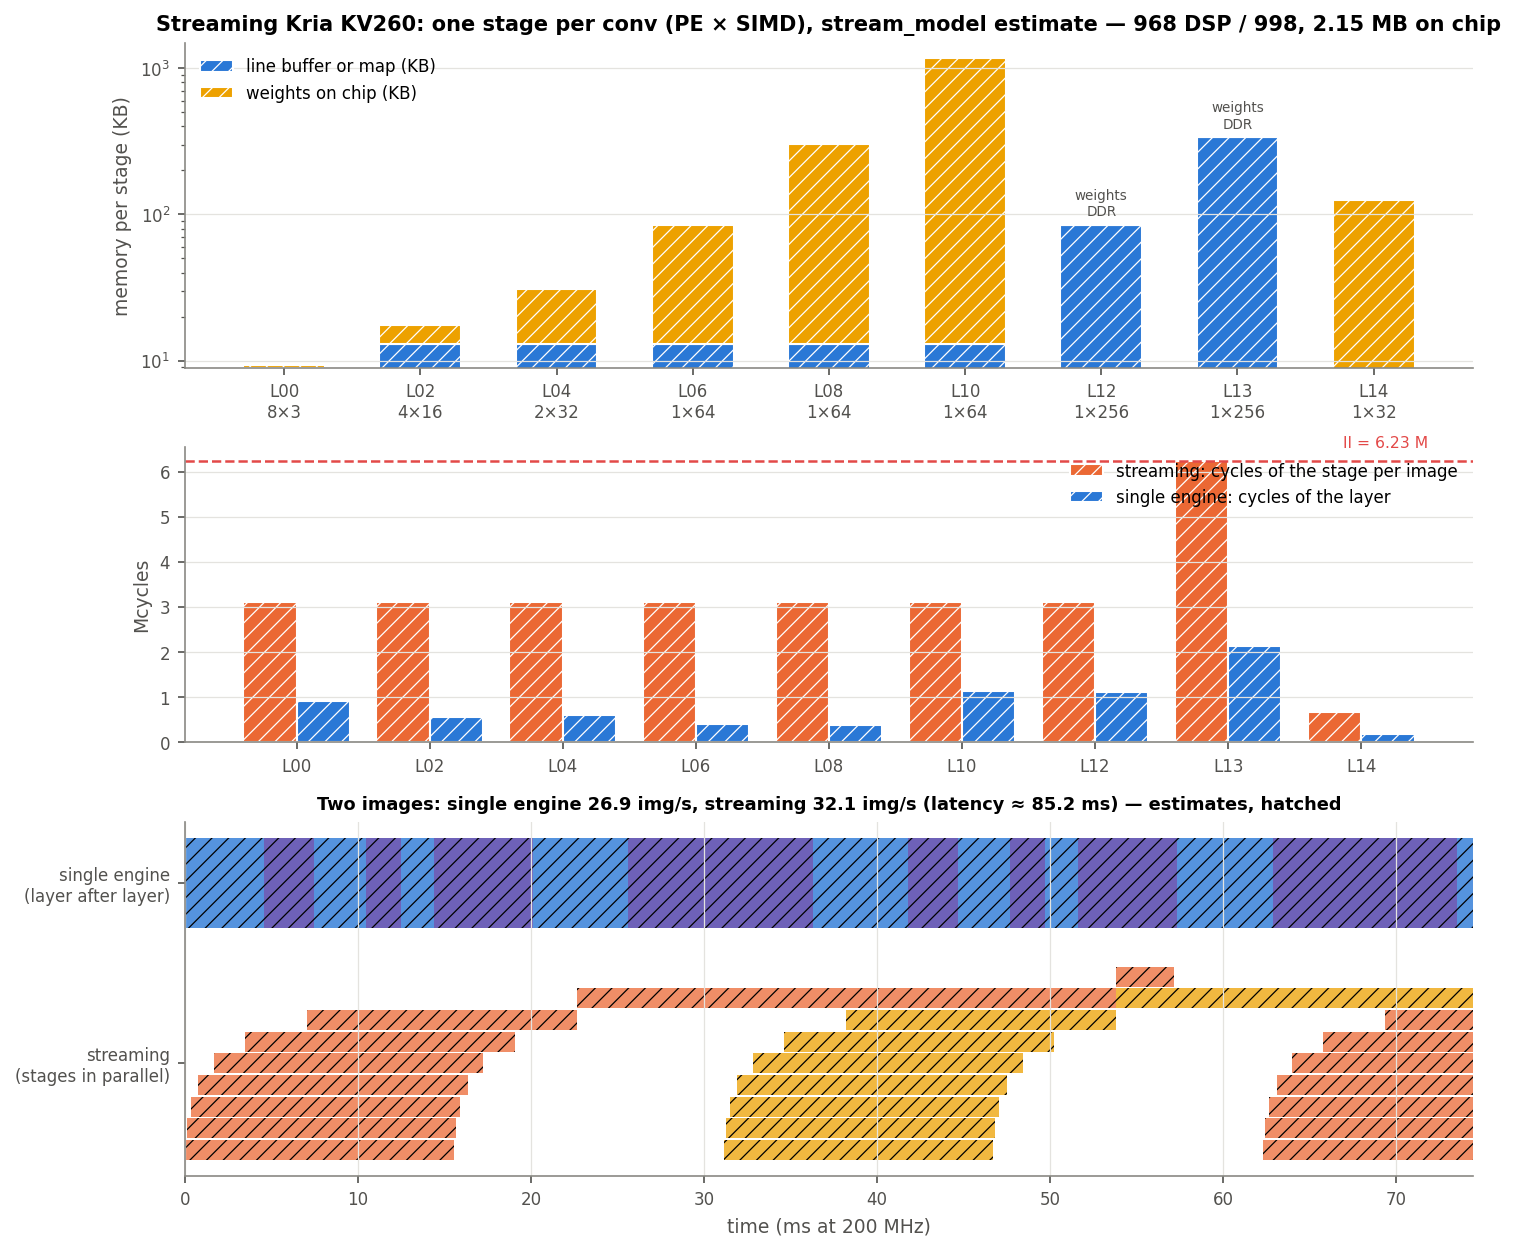
\includegraphics[width=\linewidth,height=0.42\textheight,keepaspectratio]{../../results/figures/materiel/streaming.png}
\caption{Architecture streaming face au moteur unique : mémoire et parallélisme par étage, cycles par couche, chronogramme sur deux images (estimations). (\texttt{streaming})}
\label{fig:streaming}
% python -m tools.figures streaming
\end{figure}}
\expandafter\def\csname artfig:detections\endcsname{%
\begin{figure}[htbp]
\centering
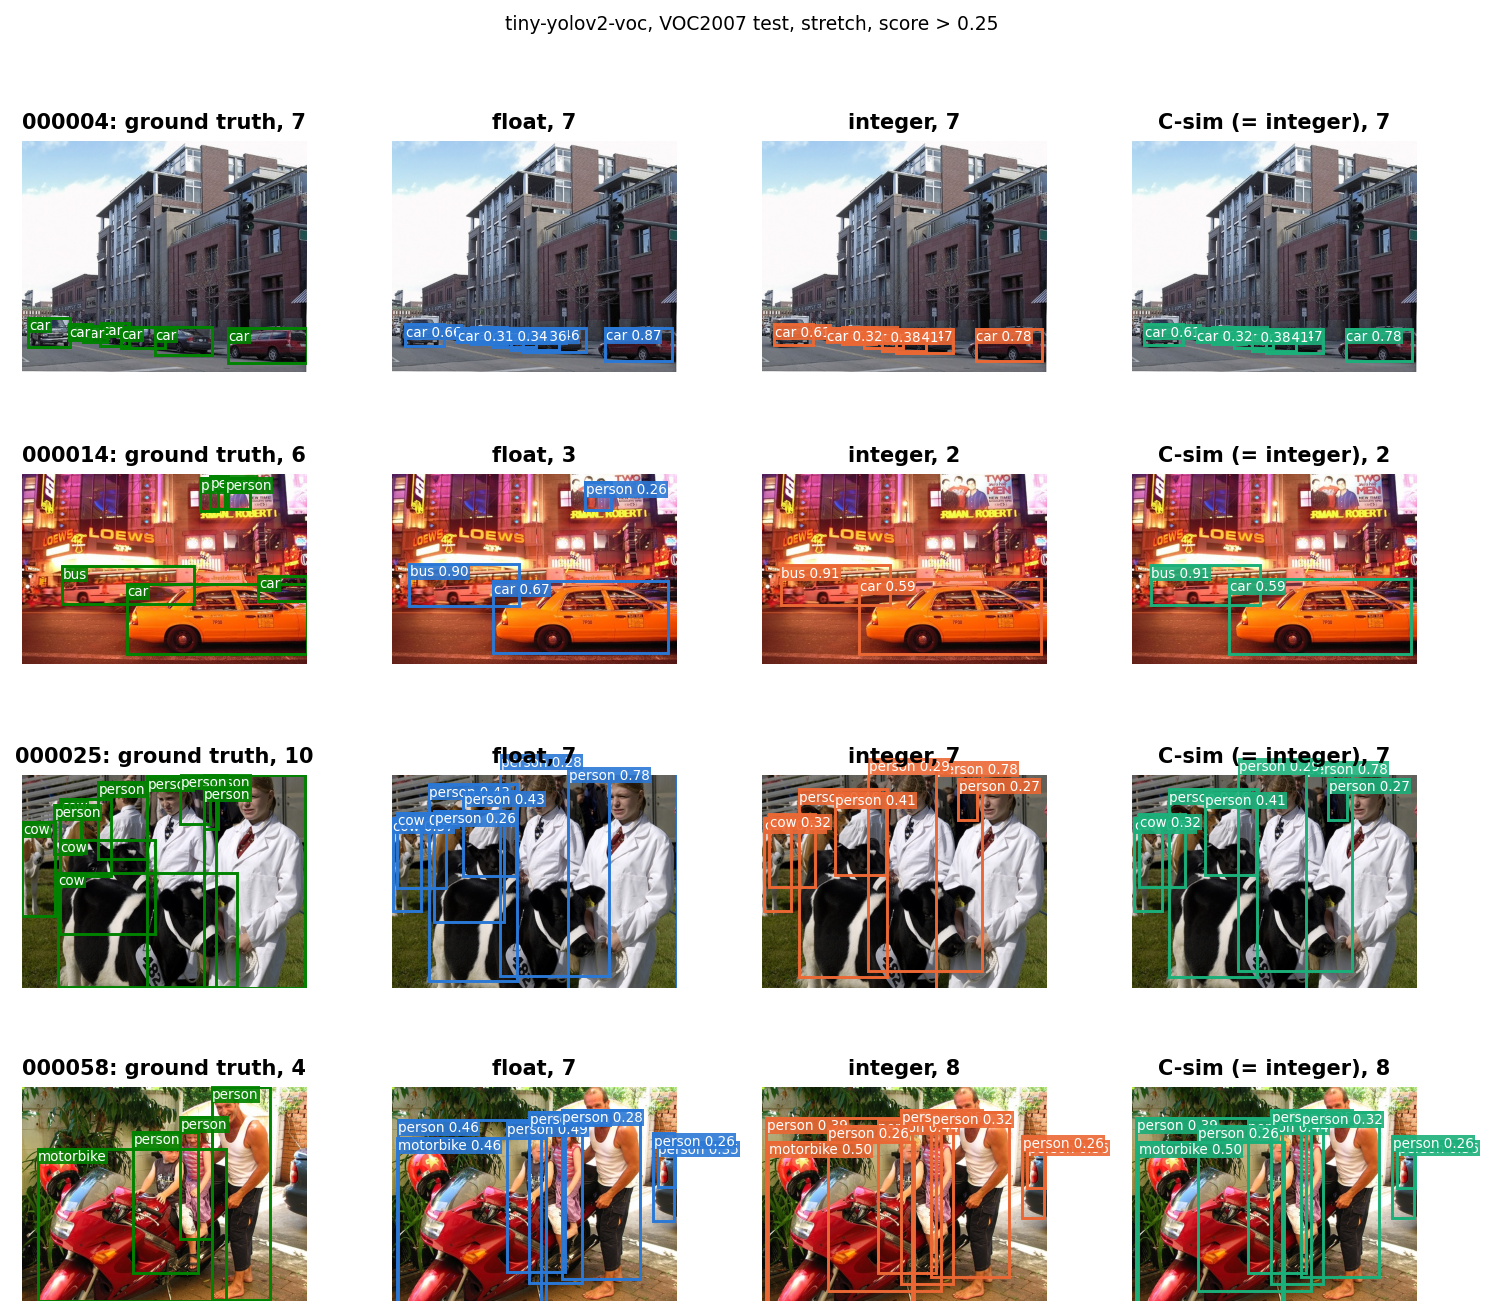
\includegraphics[width=\linewidth,height=0.42\textheight,keepaspectratio]{../../results/figures/resultats/detections.png}
\caption{Vérité terrain, flottant, entier et C-sim sur quatre images de VOC2007 test : les colonnes entier et C-sim sont identiques. (\texttt{detections})}
\label{fig:detections}
% python -m tools.figures detections
\end{figure}}
\expandafter\def\csname artfig:tests\endcsname{%
\begin{figure}[htbp]
\centering
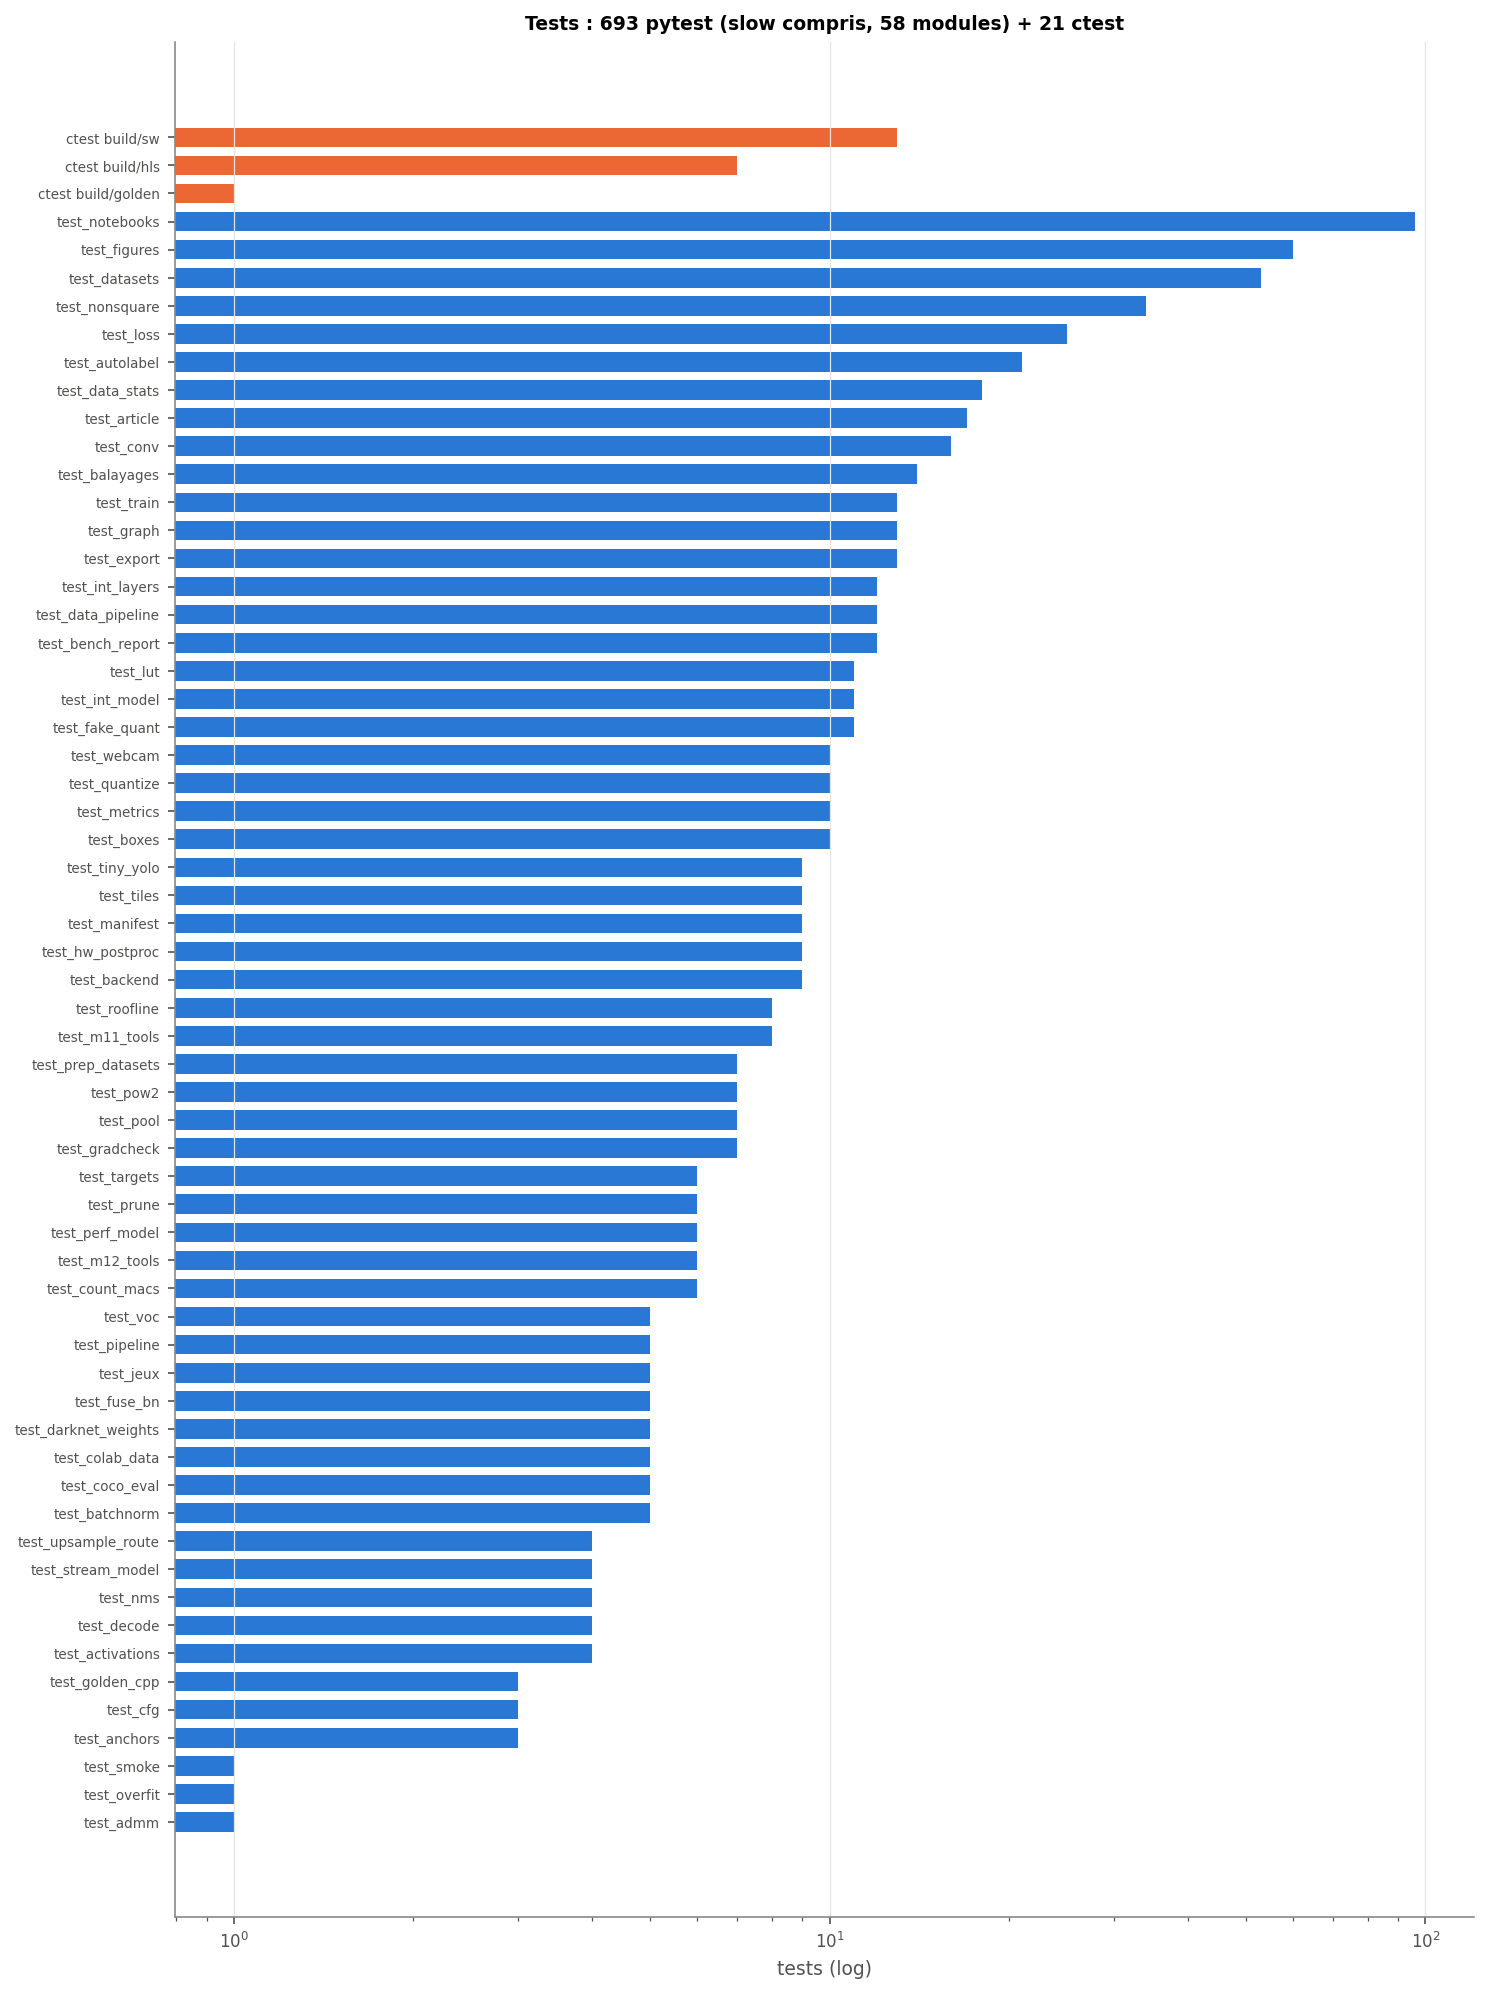
\includegraphics[width=\linewidth,height=0.42\textheight,keepaspectratio]{../../results/figures/projet/tests.png}
\caption{Nombre de tests par module Python (pytest, slow compris) et par build C++ (ctest), et leur durée quand \texttt{make test-durations} a été lancé. (\texttt{tests})}
\label{fig:tests}
% python -m tools.figures tests
\end{figure}}
\expandafter\def\csname artfig:code\endcsname{%
\begin{figure}[htbp]
\centering
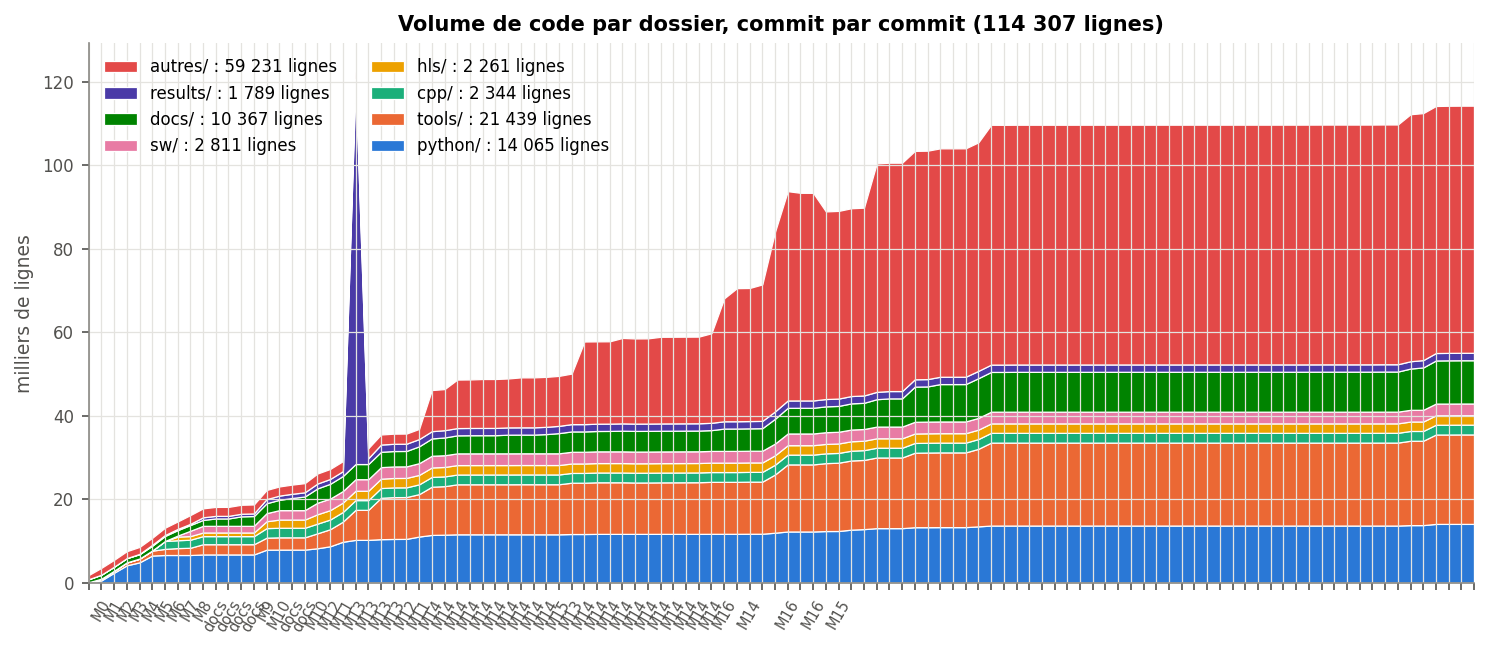
\includegraphics[width=\linewidth,height=0.42\textheight,keepaspectratio]{../../results/figures/projet/code.png}
\caption{Lignes par dossier (python, tools, cpp, hls, sw, docs, results) commit par commit. (\texttt{code})}
\label{fig:code}
% python -m tools.figures code
\end{figure}}
% ---- milestones, pending keys, revision
\newcommand\articleetat{%
\begin{tabular}{@{}lrrr@{}}
\toprule
\textbf{Milestone} & \textbf{Tasks} & \textbf{Done} & \textbf{Progress} \\
\midrule
M0 & 6 & 6 & 100\,\% \\
M1 & 9 & 8 & 89\,\% \\
M2 & 9 & 8 & 89\,\% \\
M3 & 4 & 4 & 100\,\% \\
M4 & 7 & 7 & 100\,\% \\
M5 & 6 & 6 & 100\,\% \\
M6 & 6 & 1 & 17\,\% \\
M7 & 4 & 0 & 0\,\% \\
M8 & 3 & 0 & 0\,\% \\
M9 & 1 & 0 & 0\,\% \\
M9.1 & 3 & 2 & 67\,\% \\
M9.2 & 4 & 3 & 75\,\% \\
M9.3 & 6 & 5 & 83\,\% \\
M9.4 & 3 & 3 & 100\,\% \\
M10 & 14 & 0 & 0\,\% \\
M12 & 11 & 0 & 0\,\% \\
M11 & 8 & 1 & 12\,\% \\
M13 & 54 & 54 & 100\,\% \\
M14 & 12 & 8 & 67\,\% \\
M15 & 16 & 1 & 6\,\% \\
M16 & 20 & 18 & 90\,\% \\
M17 & 21 & 17 & 81\,\% \\
M18 & 11 & 9 & 82\,\% \\
M19 & 12 & 5 & 42\,\% \\
M20 & 10 & 9 & 90\,\% \\
M21 & 12 & 6 & 50\,\% \\
M22 & 10 & 9 & 90\,\% \\
M23 & 6 & 0 & 0\,\% \\
M24 & 6 & 0 & 0\,\% \\
M25 & 6 & 0 & 0\,\% \\
M26 & 6 & 0 & 0\,\% \\
\midrule
\textbf{Total} & \textbf{306} & \textbf{190} & \textbf{62\,\%} \\
\bottomrule
\end{tabular}}
\newcommand\articleetatresume{190 of 306 tasks done across 31 milestones, 6 milestones complete}
\newcommand\articlestatuslist{%
{\raggedright
\begin{itemize}
\item \textbf{projection} (10): \texttt{perf.cascade}, \texttt{perf.kv260}, \texttt{perf.kv260.bound.ms}, \texttt{perf.kv260.m6.ms}, \texttt{perf.kv260.roofline.ms}, \texttt{perf.kv260.v2.eff}, \texttt{perf.kv260.v2.fps}, \texttt{perf.kv260.v2.gops}, \texttt{perf.kv260.v2.ms}, \texttt{perf.kv260.v3.ms}
\item \textbf{estimate} (4): \texttt{stream.w4.fps}, \texttt{stream.w8.dsp}, \texttt{stream.w8.fps}, \texttt{stream.w8.latency}
\item \textbf{tier-R} (9): \texttt{balayage.crowdhuman.meilleur.map}, \texttt{balayage.exdark.meilleur.map}, \texttt{balayage.flir.meilleur.map}, \texttt{balayage.kitti.meilleur.map}, \texttt{balayage.visdrone.meilleur.map}, \texttt{balayage.voc.meilleur.map}, \texttt{balayages.meilleurs}, \texttt{quant.sensitive.gap}, \texttt{quant.sensitive.layer}
\item \textbf{csim} (3): \texttt{map.voc.csim}, \texttt{map.voc.identical}, \texttt{verif.hwpp.cases}
\end{itemize}\par}}
\newcommand\articlerev{rev.~\texttt{66f9001-dirty}, 2026-10-19}


\graphicspath{{../../results/figures/}}
% \fig{path}{height as a fraction of the text height}
\newcommand\fig[2]{{\centering\includegraphics[width=\linewidth,height=#2\textheight,keepaspectratio]{#1}\par}}
\newcommand\src[1]{\par\vfill{\tiny\color{gray}source: \texttt{#1}}}
\newcommand\proj{\textcolor{orange!80!black}{\small(projection, not measured)}}

\title{Embedded YOLO from scratch}
\subtitle{Tiny-YOLO in NumPy, bit-exact INT8 and an HLS accelerator for the Kria KV260}
\author{Léonard Rivals}
\date{\today}

\begin{document}

\maketitle

% =====================================================================================
\section{Goal and method}

\begin{frame}{The goal}
  \footnotesize
  \begin{columns}[T]
    \column{0.55\textwidth}
    \textbf{Usual route}: train in a framework, quantize with a vendor tool, map onto a
    preconfigured unit (Vitis AI DPU). Every layer hides choices: preprocessing, rounding,
    activation, decoding.

    \medskip
    \textbf{This project takes the opposite route}: rebuild every layer by hand, so that
    every number can be traced to a line of code and checked against the stage before.
    \begin{itemize}
      \item no deep-learning library: NumPy only
      \item INT8 integer model, bit-exact down to the HLS kernel
      \item one hand-written engine for Tiny-YOLOv2, Tiny-YOLOv3 and YOLOv4-tiny
      \item dependability: faults, ABFT, OOD monitor
    \end{itemize}
    \column{0.42\textwidth}
    \begin{block}{Workloads}
      \small
      Tiny-YOLOv2 VOC: \chiffre{model.v2.mparams}\,M params, \chiffre{model.v2.gmacs} GMAC\\
      Tiny-YOLOv3: \chiffre{model.v3.mparams}\,M params, \chiffre{model.v3.gmacs} GMAC\\
      YOLOv4-tiny: \chiffre{model.v4.mparams}\,M params, \chiffre{model.v4.gmacs} GMAC\\
      YOLOv7-tiny (in progress): \chiffre{model.v7.gmacs} GMAC\\
      input $416\times416$
    \end{block}
    \begin{block}{Target}
      \small Kria KV260 (Zynq UltraScale+ XCK26), 200 MHz
    \end{block}
  \end{columns}
\end{frame}

\begin{frame}{The development chain}
  \centering
  \begin{tikzpicture}[node distance=6mm and 9mm, every node/.style={font=\small},
      box/.style={draw, rounded corners, fill=mLightBrown!15, minimum height=9mm, align=center, text width=3.3cm},
      arr/.style={-{Stealth}, thick}, chk/.style={-{Stealth}, thick, dashed, mLightGreen!80!black}]
    \node[box] (py) {\texttt{python/}\\float model};
    \node[box, right=of py] (int) {bit-exact\\integer model};
    \node[box, right=of int] (exp) {\texttt{model/}\\manifest + blobs + dumps};
    \node[box, below=12mm of py] (gold) {\texttt{cpp/golden/}\\tiled C++ engine};
    \node[box, right=of gold] (hls) {\texttt{hls/}\\Vitis HLS kernel};
    \node[box, right=of hls] (sw) {\texttt{sw/}\\ARM driver + post-proc.};
    \draw[arr] (py) -- (int);
    \draw[arr] (int) -- node[above]{export} (exp);
    \draw[chk] (exp) -- node[sloped, above, font=\scriptsize]{layer by layer} (gold);
    \draw[chk] (exp) -- node[right, font=\scriptsize]{C-sim / co-sim} (hls);
    \draw[chk] (exp) -- node[right, font=\scriptsize, pos=0.6]{board} (sw);
  \end{tikzpicture}

  \bigskip
  \raggedright
  Each hand-over is checked for \textbf{equality of bytes}, not closeness. Specification:
  \texttt{yolo-embarque-de-zero.md}; decisions: 3 ADRs (pure NumPy, HLS, board choice).
\end{frame}

\begin{frame}{Work plan}
  \begin{columns}[T]
    \column{0.5\textwidth}
    \tiny
    \begin{description}[M9.x]
      \item[M0--M3] NumPy building blocks, loss, training, inference, float mAP
      \item[M4--M5] INT8 quantization, golden C++
      \item[M6--M8] HLS accelerator, SoC, measurements
      \item[M9.x] HW post-processing, REQ-YOLO, 4 bits, streaming
      \item[M10] kernel optimisation cascade
      \item[M11--M18] datasets, PC profiles, figures, notebooks, Colab campaign, article
      \item[M19--M22] English, webcam demo, ASL, auto-labeller
      \item[M23--M26] two MACs per DSP, YOLOv4-tiny, dependability, recent models
      \item[M27--M31] safety: metrics, equivalence, monitors, latency bound, assurance
      \item[M32--M36] TrashNet, Pet; v5n, v7-tiny, v8n without PyTorch; explanation
    \end{description}
    \column{0.48\textwidth}
    \fig{projet/chronologie.png}{0.6}
  \end{columns}
  \raggedright\small State at the last render: \articleetatresume.
\end{frame}

\begin{frame}{Progress by milestone}
  \begin{columns}[T]
    \column{0.40\textwidth}
    \centering\tiny\renewcommand\arraystretch{0.68}%
    \scalebox{0.72}{\articleetat}
    \column{0.58\textwidth}
    \fig{projet/avancement.png}{0.75}
  \end{columns}
\end{frame}

% =====================================================================================
\section{From scratch in NumPy (M0--M3)}

\begin{frame}{The networks}
  \begin{columns}[c]
    \column{0.62\textwidth}
    \fig{reseaux/flux_tiny-yolov2-voc.png}{0.33}
    \fig{reseaux/flux_tiny-yolov3-coco.png}{0.38}
    \column{0.36\textwidth}
    \small
    \textbf{Tiny-YOLOv2}: 9 conv $3\times3$ + BN + leaky ReLU, 6 max-pools, linear
    $1\times1$ head with $5\times(5+C)$ filters.

    \medskip
    \textbf{Tiny-YOLOv3}: a second head at $26\times26$ fed by upsample + route.

    \medskip
    Counted by \texttt{make count-macs} from the network descriptions.
  \end{columns}
\end{frame}

\begin{frame}{YOLOv4-tiny and YOLOv7-tiny (M24, M26)}
  \begin{columns}[c]
    \column{0.62\textwidth}
    \fig{reseaux/flux_tiny-yolov4-coco.png}{0.78}
    \column{0.36\textwidth}
    \small
    \textbf{YOLOv4-tiny}: CSP blocks; a \emph{grouped route} reads half of the channels
    of a map (one more addressing mode, no copy); \texttt{scale\_x\_y} on the box centres.

    \medskip
    \textbf{YOLOv7-tiny} (in progress): ELAN blocks with 4-source concatenations, SPP with
    stride-1 pools $5/9/13$, exported as chained $5\times5$ pools. Float, calibration and
    export done; accuracy not measured yet.
  \end{columns}
\end{frame}

\begin{frame}{Layers with forward and backward passes}
  \fig{maths/convolution.png}{0.32}
  \fig{maths/retropropagation.png}{0.33}
  \footnotesize Interface \texttt{forward(x) -> (y, cache)}, \texttt{backward(dy, cache) -> (dx, grads)}.
  Naive and im2col convolutions agree to $10^{-12}$; every layer passes a float64
  finite-difference gradient check (max norm).
\end{frame}

\begin{frame}{Targets, loss and training}
  \begin{columns}[c]
    \column{0.58\textwidth}
    \fig{maths/perte.png}{0.78}
    \column{0.4\textwidth}
    \small
    \begin{itemize}
      \item YOLOv3 loss: box offset regression, logistic objectness with an
        \emph{ignore} rule, multi-label BCE for the classes
      \item targets on the best anchor (IoU of shapes); anchors by k-means with
        $1-\mathrm{IoU}$
      \item SGD, burn-in, multi-scale inputs
      \item \textbf{one image overfitted}: targets, loss and optimiser validated together
    \end{itemize}
  \end{columns}
\end{frame}

\begin{frame}{Anchors from k-means}
  \fig{modeles/ancres.png}{0.55}
  \fig{maths/kmeans.png}{0.25}
\end{frame}

\begin{frame}{Inference and VOC evaluation}
  \begin{columns}[c]
    \column{0.5\textwidth}
    \fig{maths/nms_map.png}{0.28}
    \footnotesize
    \begin{itemize}
      \item YOLOv2 decoding, per-class NMS at IoU 0.45
      \item VOC2007 protocol: 11-point AP, \texttt{difficult} ignored; matches the
        official devkit to $10^{-12}$
    \end{itemize}
    \column{0.48\textwidth}
    \scriptsize\articletable{map.voc.float.table}
  \end{columns}
  \footnotesize Float reference with Darknet weights: \textbf{\chiffre{map.voc.float}} mAP, against
  \chiffre{map.voc.darknet} published. Preprocessing matters: a letterbox loses $\approx 2$
  points with these weights, so the reference uses the direct resize (also the simplest
  in hardware).
\end{frame}

\begin{frame}{Precision--recall by preprocessing}
  \fig{resultats/pr_variantes.png}{0.85}
\end{frame}

\begin{frame}{COCO val2017 (M24)}
  \begin{minipage}{\linewidth}\scriptsize\articletable{map.coco.table}\end{minipage}
  \begin{columns}[c]
    \column{0.55\textwidth}
    \footnotesize
    COCO metric, equal to \texttt{pycocotools} to $10^{-4}$. YOLOv4-tiny:
    \textbf{\chiffre{map.coco.v4.ap50}} AP50 (published \chiffre{map.coco.v4.published} on
    test-dev). Tiny-YOLOv3 is optimistic: val2017 overlaps its COCO 2014 training images.

    \medskip
    INT8: \chiffre{map.coco.v4.int8.ap50} AP50, \textbf{\chiffre{map.coco.v4.drop}} point,
    above the one-point target; the loss is spread over the backbone, QAT open.
    \column{0.43\textwidth}
    \fig{resultats/map_coco.png}{0.42}
  \end{columns}
\end{frame}

% =====================================================================================
\section{INT8 quantization (M4)}

\begin{frame}{An integer-only network}
  \fig{maths/quantification.png}{0.25}
  \fig{maths/entier.png}{0.25}
  \footnotesize
  \begin{itemize}
    \item BN folded into the weights; weights per output channel, activations per layer
      (\texttt{p99.99} of $|x|$ on 500 images, MSE criterion)
    \item 32-bit accumulator, requantization by an integer multiplier $M_0$ and a shift:
      \textbf{no floating point left}
    \item leaky slope $13/128$ as $(13y+64)\gg7$ (rounding, not flooring: no bias
      accumulating across layers); sigmoid and exp by 256-entry tables, step $1/8$
  \end{itemize}
\end{frame}

\begin{frame}{Calibration}
  \fig{resultats/calibration_tiny-yolov2-voc.png}{0.85}
\end{frame}

\begin{frame}{Accuracy of the integer model}
  \begin{columns}[c]
    \column{0.45\textwidth}
    \scriptsize\articletable{map.voc.int8.table}

    \medskip\small
    Drop of \textbf{\chiffre{map.voc.drop}} point: below the one-point target, no QAT needed.
    Most sensitive layer alone: \chiffre{quant.sensitive.layer}
    (\chiffre{quant.sensitive.gap}), within subset noise: the loss is spread out.
    \column{0.53\textwidth}
    \fig{resultats/erreur_couches_tiny-yolov2-voc.png}{0.75}
  \end{columns}
\end{frame}

% =====================================================================================
\section{Golden model and verification (M5)}

\begin{frame}{A C++ golden model that runs like the hardware}
  \footnotesize
  The quantized network is exported as a manifest + binary blobs, with the integer
  activations of every layer on a few images (dumps). The C++17 golden model reads the same
  export and runs it \emph{as the hardware will}: tiled convolution with fixed buffers,
  bias, requantization, leaky + fused max-pool, route by addressing.

  \medskip
  \fig{materiel/chaine_verif.png}{0.24}

  \begin{itemize}
    \item \texttt{make golden-check}: \chiffre{verif.dumps} dumps compared layer by layer
    \item \texttt{make csim-gcc}: HLS kernel == golden; \texttt{make sw-sim}: ARM driver == golden
    \item all of it in \texttt{make ci} on every commit (synthetic export without weights)
  \end{itemize}
\end{frame}

\begin{frame}{Tests}
  \begin{columns}[c]
    \column{0.55\textwidth}
    \fig{projet/tests.png}{0.85}
    \column{0.43\textwidth}
    \small
    \begin{itemize}
      \item pytest (NumPy layers, gradcheck, metrics, tools)
      \item Catch2 for the golden model
      \item C-sim with \texttt{g++} for the HLS kernels
      \item tiers R / M / N (M12): rapid, medium, night runs, each with a criterion and a
        decision
    \end{itemize}
  \end{columns}
\end{frame}

% =====================================================================================
\section{HLS accelerator and SoC (M6--M7)}

\begin{frame}{Choosing the board before writing HLS}
  \begin{columns}[c]
    \column{0.55\textwidth}
    \fig{resultats/roofline_couches_kv260.png}{0.72}
    \column{0.43\textwidth}
    \small
    A roofline explorer (\texttt{make roofline}) over the candidate boards (PYNQ-Z2,
    Zybo Z7-20, Ultra96-v2, KV260).

    \medskip
    \textbf{ADR 0003}: the KV260 gives about \textbf{6$\times$} the roofline performance of a
    Zynq-7020 board for these networks, at the same price.
  \end{columns}
\end{frame}

\begin{frame}{One engine, layer by layer}
  \begin{columns}[c]
    \column{0.52\textwidth}
    \fig{materiel/moteur.png}{0.75}
    \column{0.46\textwidth}
    \fig{materiel/tuilage.png}{0.45}
    \footnotesize
    Loop nest tiled over output/input channels, rows and columns:
    $T_m=32$, $T_n=24$, $T_r=T_c=13$ $\Rightarrow$ \textbf{768 MAC/cycle} at 200 MHz.
    Upsample and route cost no compute: they change the read address of the next layer.
  \end{columns}
\end{frame}

\begin{frame}{SoC integration}
  \begin{columns}[c]
    \column{0.55\textwidth}
    \fig{materiel/soc.png}{0.75}
    \column{0.43\textwidth}
    \small
    \begin{itemize}
      \item ARM loads manifest + blobs in contiguous memory, programs the AXI-Lite
        registers layer after layer, waits for the interrupt
      \item block design, device-tree overlay and firmware are scripted
        (\texttt{make vivado-build}, \texttt{fpga-firmware})
      \item \textbf{not run yet}: Vivado/Vitis and the board are not available; everything
        above the hardware runs on the PC through a simulation backend
    \end{itemize}
  \end{columns}
\end{frame}

% =====================================================================================
\section{Results (M8)}

\begin{frame}{mAP at the three stages of the chain}
  \begin{columns}[c]
    \column{0.6\textwidth}
    \scriptsize\articletable{map.stades}
    \column{0.38\textwidth}
    \fig{resultats/map_stades.png}{0.6}
  \end{columns}
  \small On the \textbf{\chiffre{map.voc.images} images} of VOC2007 test, the ARM driver over
  the C-simulated kernel gives detections \textbf{identical} to the Python integer model:
  the whole accuracy loss comes from quantization.
\end{frame}

\begin{frame}{Projected performance on the KV260 \proj}
  \footnotesize\articletable{perf.kv260}

  \medskip\small
  Tiny-YOLOv2: \textbf{\chiffre{perf.kv260.v2.ms}\,ms}, \chiffre{perf.kv260.v2.fps} img/s,
  \chiffre{perf.kv260.v2.gops} GOPS, efficiency \chiffre{perf.kv260.v2.eff}\,\%.
  The cycle model \texttt{tools/perf\_model.py} equals the C-sim counters cycle for cycle;
  it is a lower bound (II = 1, no pipeline depth, DDR latency or ARM control).
\end{frame}

\begin{frame}{Against the state of the art}
  \fig{resultats/etat_art.png}{0.5}
  \small
  \begin{itemize}
    \item \textbf{2024-zhang}, only reference on the same model: two MACs per DSP and HW
      post-processing; packing (M23) closes the multiplier gap
    \item same board as \textbf{2026-fata} (Vitis AI DPU, 70\,\% pruning, QAT): the projected
      kernel exceeds it in img/s \emph{without pruning}
  \end{itemize}
\end{frame}

% =====================================================================================
\section{Kernel optimisation (M10)}

\begin{frame}{From \chiffre{perf.kv260.m6.ms} to \chiffre{perf.kv260.v2.ms} ms \proj}
  \begin{columns}[c]
    \column{0.6\textwidth}
    \fig{resultats/cascade_m10.png}{0.75}
    \column{0.38\textwidth}
    \small
    The M6 kernel spent most of its cycles outside the MAC loop, waiting for its 8-bit
    ports and its output stage.

    \medskip
    Each step of the cascade stays C-sim equal to the golden model.
  \end{columns}
\end{frame}

\begin{frame}{The optimisation cascade, step by step \proj}
  \scriptsize\articletable{perf.cascade}
\end{frame}

\begin{frame}{Where the cycles go now}
  \begin{columns}[c]
    \column{0.6\textwidth}
    \fig{resultats/cycles_couches.png}{0.8}
    \column{0.38\textwidth}
    \small
    64-bit ports, valid input channels only, 8 channels requantized per cycle, first layer
    folded onto the input lanes, $14\times14$ tiles for pooled convolutions.

    \medskip
    Compute bound \chiffre{perf.kv260.bound.ms}\,ms, roofline point
    \chiffre{perf.kv260.roofline.ms}\,ms.
  \end{columns}
\end{frame}

\begin{frame}{Two INT8 MACs per DSP (M23)}
  \begin{columns}[c]
    \column{0.5\textwidth}
    \fig{materiel/dsp_packing.png}{0.6}
    \column{0.48\textwidth}
    \scriptsize
    \begin{itemize}
      \item weights of two output channels in the 27-bit port: $A = w_a 2^{18} + w_b$, one
        product gives both
      \item exact for 8 accumulated products under the $\pm127$ contract: the 24-lane tree
        is cut into $3\times8$
      \item only the multiplication changes: C-sim == golden \textbf{to the byte}, cycles
        unchanged
      \item same tiles: half the DSPs; $T_m=64$: \chiffre{pack.v2.tm64.ms}\,ms (flip-flops
        over budget); $T_n=32$: \chiffre{pack.v2.tn32.ms}\,ms \proj
    \end{itemize}
  \end{columns}
\end{frame}

\begin{frame}{Packed PE options \proj}
  \tiny\articletable{pack.table}
\end{frame}

\begin{frame}{Packed PE options per network \proj}
  \fig{resultats/pack_options.png}{0.85}
\end{frame}

\begin{frame}{Winograd against packing}
  \begin{columns}[c]
    \column{0.66\textwidth}
    \fig{resultats/winograd.png}{0.8}
    \column{0.32\textwidth}
    \footnotesize
    Integer-exact $F(2\times2,3\times3)$: fewer multiplications on the $3\times3$ convs,
    slightly ahead on the compute bound alone.

    \medskip
    With the loads it loses: wider transformed weights consumed faster, a weight buffer
    beyond the flip-flops of the board, and products that do not pack two to a DSP.
    \textbf{Studied, not implemented.}
  \end{columns}
\end{frame}

% =====================================================================================
\section{Research extensions (M9)}

\begin{frame}{Hardware post-processing (M9.1)}
  \fig{resultats/hw_postproc.png}{0.4}
  \small
  \begin{itemize}
    \item a second HLS kernel decodes the heads and runs the NMS \textbf{in integers only}:
      threshold on the integer logit, one reciprocal per cell, Q4 pixel corners, IoU as an
      integer inequality, 256 slots in stream order, no sort
    \item \chiffre{map.formats.hwpp} mAP; equal to its golden mirror on
      \chiffre{verif.hwpp.cases} cases; synthesis pending
  \end{itemize}
\end{frame}

\begin{frame}{Formats on the same model (M9.2, M9.3)}
  \begin{columns}[c]
    \column{0.56\textwidth}
    \scriptsize\articletable{map.formats}
    \column{0.42\textwidth}
    \fig{resultats/map_formats.png}{0.4}
    \scriptsize
    \textbf{REQ-YOLO}: weights as sums of two powers of two, no DSP for MACs; projection
    \chiffre{map.formats.mixed6}, ADMM \emph{did not converge} (\chiffre{map.formats.admm}).\\
    \textbf{W4A4}: PTQ \chiffre{map.formats.w4a4.ptq} $\to$ short QAT
    \chiffre{map.formats.w4a4.qat} (loss still decreasing). Both exports are bit-exact in
    golden and C-sim.
  \end{columns}
\end{frame}

\begin{frame}{Streaming architecture (M9.4)}
  \begin{columns}[c]
    \column{0.5\textwidth}
    \fig{materiel/streaming.png}{0.8}
    \column{0.48\textwidth}
    \small
    One stage per convolution with line buffers. The weights of Tiny-YOLOv2 do not fit on
    chip: a \textbf{hybrid} plan, the two largest layers read theirs from DDR once per image.

    \medskip
    Estimates: \chiffre{stream.w8.fps} img/s with \chiffre{stream.w8.dsp} DSP, latency
    \chiffre{stream.w8.latency}\,ms; \chiffre{stream.w4.fps} img/s with 4-bit weights.
    The streaming kernel equals the golden model stage by stage in C-sim.
  \end{columns}
\end{frame}

\begin{frame}{Resources: single engine vs streaming}
  \fig{resultats/ressources.png}{0.65}
  \small Roofline model for the single engine (896 DSP, 112 BRAM18) against the streaming
  plan. Real resources will only be known after synthesis.
\end{frame}

% =====================================================================================
\section{Dependability (M25)}

\begin{frame}{Faults and an exact checksum}
  \small
  The bit-exact integer model is a fault-free reference: any difference is caused by the
  injected fault.
  \begin{itemize}
    \item \textbf{Injector}: bit flips (given bit or error rate) and stuck-at in INT8
      weights, int32 biases, INT8 activations, int32 accumulator; seeded; no fault $=$
      integer model exactly
    \item \textbf{Campaign}: mAP against error rate, layer and bit position; smoke run only,
      full grids to run
    \item \textbf{ABFT}: sum of the output channels $=$ conv of the input by the summed
      filters. All integer before requantization $\Rightarrow$ \textbf{exact modulo
      $2^{32}$}, no tolerance, no false alarm
    \item in the integer model, the golden model and the \textbf{HLS kernel} (one more
      lane, C-sim): 0 false alarm on 103 layers and 158 outputs, every accumulator fault
      detected; its synthesis cost waits for Vitis
  \end{itemize}
\end{frame}

\begin{frame}{Out-of-distribution monitor}
  \footnotesize
  Reads the INT8 output of the last backbone layer of Tiny-YOLOv2 (already written by the
  accelerator), scored on the ARM.
  \begin{itemize}
    \item dark and thermal images give \emph{weaker} features: they fall inside the
      in-domain shell, so raw distances are \emph{lower} out of domain
    \item the monitor uses the \textbf{typicality} of the score: distance to the median on
      held-out VOC images, in either direction
    \item the plain feature norm wins: AUROC \chiffre{ood.norm.auroc.exdark} (low light),
      \textbf{\chiffre{ood.norm.auroc.flir}} (thermal), for a negligible share of the MACs
  \end{itemize}
  \medskip
  \scriptsize\articletable{ood.table}
\end{frame}

% =====================================================================================
\section{Safety evidence (M28, M30)}

\begin{frame}{Model $\leftrightarrow$ circuit equivalence (M28)}
  \small
  Three levels of evidence: \textbf{pointwise} (same output), \textbf{bounded
  proximity}, \textbf{statistical}, stage by stage, on the four exports.
  \begin{itemize}
    \item integer $\to$ golden $\to$ C-sim: \textbf{pointwise}, every byte of every layer
      output, the ABFT check silent
    \item fake-quant $\to$ integer: $\le 1$ LSB per layer (bounded proximity, measured);
      float $\to$ integer: \chiffre{map.voc.drop} mAP (statistical)
    \item exhaustive operator tests (Python $=$ golden $=$ HLS), a z3 proof of the scalar
      kernels, per-layer traceability checked in \texttt{make ci}
    \item post-processing: NMS $=$ golden; capacity and overflow properties hold, the
      unsorted NMS depends on the order of the cells
    \item co-sim and board rows: pending (Vitis, KV260)
  \end{itemize}
  \src{results/equivalence.md}
\end{frame}

\begin{frame}{A latency bound that does not depend on the image (M30)}
  \small
  \begin{itemize}
    \item the engine runs a fixed schedule of layer descriptors: every loop bound comes
      from the descriptor, activations and weights are never a condition $\Rightarrow$ the
      cycle count of a layer is a function of its shape only
    \item the \textbf{static bound} gives up every overlap and adds DDR traffic and burst
      latency: Tiny-YOLOv2 accelerator \textbf{83.4\,ms}, whole frame with the
      post-processing \textbf{92\,ms} \proj
    \item the post-processing is the data-dependent part, bounded by its 256 slots;
      adversarial C-sim cases stay under the bound
    \item the uncapped NMS of sigmoid heads dominates v3 and v4-tiny
    \item next: cycle distribution over $\ge$ 10,000 real images, then p99.9 and jitter on
      the board
  \end{itemize}
  \src{results/latency\_bound.md}
\end{frame}

% =====================================================================================
\section{Beyond VOC (M11--M18, M21)}

\begin{frame}{Datasets, each chosen to stress one part of the chain}
  \small
  \begin{columns}[T]
    \column{0.5\textwidth}
    \begin{description}[CrowdHuman]
      \item[COCO] 80 classes, Tiny-YOLOv3 weights
      \item[VisDrone] aerial, tiny objects
      \item[KITTI] driving, wide images
      \item[FLIR] thermal, 1 channel
      \item[ExDark] low light
      \item[CrowdHuman] crowds, grid collisions
    \end{description}
    \column{0.48\textwidth}
    \begin{description}[DroneVehicle]
      \item[AU-AIR] 1080p frames, class imbalance
      \item[DroneVehicle] oriented $\to$ upright boxes
      \item[HIT-UAV] thermal from 60--130 m
      \item[UAVDT] $1024\times540$ video frames
      \item[ASL] classification $\to$ detection with MediaPipe hand pseudo-boxes
        (87.5\,\% of images get a box)
    \end{description}
  \end{columns}
  \medskip
  Per dataset: loader, datasheet, statistics notebook (M16: classes, box sizes, density,
  anchors, collisions in the grid), archive on Google Drive (rclone) for Colab.
\end{frame}

\begin{frame}{Notebooks and the Colab campaign (M14, M15)}
  \small
  \begin{itemize}
      \item \texttt{make notebooks}: inference, training and sweep (batch $\times$ subset)
        per model $\times$ dataset, generated from templates; they only call repository
        code
      \item run locally or on a Colab GPU from VS Code; outputs synced to Drive and
        harvested back (\texttt{make harvest})
      \item first sweeps: 600 iterations, scored on 50 images (tier R): \emph{ranking}, not
        published results; none of these runs has converged yet
  \end{itemize}
\end{frame}

\begin{frame}{Best run of the first sweep of each dataset \textcolor{orange!80!black}{\small(tier R)}}
  \scriptsize\articletable{balayages.meilleurs}
\end{frame}

\begin{frame}{Detections}
  \fig{resultats/detections.png}{0.8}
\end{frame}

% =====================================================================================
\section{Tooling and demos (M13, M17, M19--M22)}

\begin{frame}{Everything is regenerated}
  \begin{columns}[c]
    \column{0.5\textwidth}
    \small
    \begin{itemize}
      \item \textbf{M13}: 88 figures by \texttt{make figures} (models, accelerator,
        results, project, the maths of the reimplementation)
      \item \textbf{M17}: a paper-style article; \texttt{make article} collects every number
        with its status (measured, C-sim, projection, estimate, tier R) --- this deck uses
        the same macros
      \item \textbf{M19}: docs, spec and generated text in English, checked in
        \texttt{make ci}
    \end{itemize}
    \column{0.48\textwidth}
    \fig{projet/code.png}{0.4}
    \fig{projet/dependances.png}{0.3}
  \end{columns}
\end{frame}

\begin{frame}{Live webcam demo (M20)}
  \small
  \begin{columns}[c]
    \column{0.55\textwidth}
    \begin{itemize}
      \item \texttt{make webcam}: pick a model (float or integer, VOC or COCO), live camera
        image, continuous inference, boxes and classes on screen
      \item capture thread at the camera rate (20 FPS measured), inference thread at
        3--5 FPS on the CPU ($\approx 200$\,ms): boxes and image always match
      \item same pipeline as \texttt{tools/detect.py}: \texttt{preprocess} $\to$
        \texttt{detect}/\texttt{detect\_int} $\to$ \texttt{draw}
      \item outlook: the same demo on the KV260 with the accelerator
    \end{itemize}
    \column{0.42\textwidth}
    \begin{block}{Commands}
      \scriptsize\ttfamily
      make get-weights\\
      python tools/webcam.py --list\\
      make webcam\\
      python tools/webcam.py \textbackslash\\
      \quad --model int:tiny-yolov2-voc
    \end{block}
  \end{columns}
\end{frame}

\begin{frame}{Photo auto-labelling (M22)}
  \small
  \begin{columns}[c]
    \column{0.55\textwidth}
    \begin{itemize}
      \item \texttt{make autolabel}: drag \& drop a photo or a folder, classes typed as
        text
      \item open-vocabulary labellers: Grounding DINO tiny (default), OWLv2
      \item manual correction in the browser, export as YOLO txt (one file, or a zip)
      \item purpose: build training sets for new classes, fine-tune the embedded
        Tiny-YOLO, run it on the webcam or the board
    \end{itemize}
    \column{0.42\textwidth}
    \begin{block}{Idea}
      Generalises the ASL pseudo-boxes (M21) from hands to any class that can be named.
      The large labeller never goes on the FPGA.
    \end{block}
  \end{columns}
\end{frame}

% =====================================================================================
\section{Conclusion}

\begin{frame}{Limitations and next steps}
  \scriptsize
  \begin{itemize}
    \item \textbf{No number is measured on the board yet}: performance is a cycle-model
      projection, resources are estimates, the FPGA mAP is a C simulation $\to$ synthesis,
      co-sim and board runs (M6--M8), then \texttt{run\_compare} must show 0 differences
    \item REQ-YOLO ADMM did not converge; the 4-bit QAT ran for a fraction of an epoch
    \item NumPy training from scratch (VOC fine-tuning, M2) is not finished: the reference
      uses Darknet weights
    \item datasets beyond VOC explored at tier R only: longer runs, matching resize, tiles
      (M15)
    \item YOLOv4-tiny: full C-sim pass on COCO and QAT; YOLOv7-tiny accuracy; YOLOv5n,
      YOLOv8n trained without PyTorch (M33--M35)
    \item fault campaign at full size; person metrics, runtime monitors and the assurance
      case (M27, M29, M31) wait for CrowdHuman on the PC; explanation planned (M36)
    \item the open runs ($\approx$\,40\,h CPU, 12\,h C-sim, 110--120\,h GPU) are listed in
      \texttt{docs/tasks/long-runs.md} and scheduled in \texttt{status.pdf}
  \end{itemize}
  \medskip
  Every projected or estimated value carries its status in the slides; T17.19 switches
  them to measurements once the board runs.
\end{frame}

\begin{frame}{Summary}
  \small
  \begin{itemize}
    \item A complete detection chain \textbf{without a learning library}, every gradient checked
    \item \textbf{Bit-exact} from the NumPy integer model to the C-simulated HLS kernel behind
      the ARM driver, on the full VOC2007 test set:
      \chiffre{map.voc.float} $\to$ \chiffre{map.voc.int8} $\to$ \chiffre{map.voc.csim} mAP
    \item \textbf{One engine} for v2, v3 and YOLOv4-tiny, projected at
      \chiffre{perf.kv260.v2.ms}\,ms per image on the KV260
      (\chiffre{pack.v2.tm64.ms}\,ms with two MACs per DSP)
    \item \textbf{Dependability}: exact int32 ABFT, fault injection, an OOD monitor almost
      for free
    \item \textbf{Safety evidence}: model $\leftrightarrow$ circuit equivalence per layer,
      proved scalar kernels, a latency bound independent of the image
    \item INT8, power-of-two, 4-bit and integer post-processing \textbf{compared on the same
      model}
    \item \textbf{Reproducible}: tests, figures, notebooks, article and these slides
      regenerated by \texttt{make}
  \end{itemize}
\end{frame}

\begin{frame}[standout]
  Questions?
\end{frame}

\end{document}
